Rapid advances in artificial intelligence, particularly in the field of large language models (LLMs), have had a significant impact on the development of AI chatbots. These models, powered by complex architectures and vast datasets, have demonstrated remarkable natural language processing capabilities, enabling more sophisticated, human-like interactions. However, the evolution of these models is not without challenges, particularly with regard to scalability, training, and application in different contexts.

This chapter reviews the technical foundations and advances that have shaped the current state of LLMs, with a specific emphasis on the Transformer architecture, which has been instrumental in the success of these models. The chapter examines the evolution of LLMs, their architectural components, and the impact of model size on performance. In addition, the chapter examines the training processes underlying these models, including the pre-training and tuning techniques that have become essential to optimizing their performance in specific tasks.

In addition, the chapter addresses the Retrieval-Augmented Generation (RAG) paradigm, which enhances the capabilities of AI chatbots by integrating information retrieval processes. This approach not only improves the factual accuracy of generated content, but also facilitates the personalization of responses based on external knowledge sources.

The final section of the chapter will examine the limitations of contemporary LLMs in practical applications, analyzing the shortcomings of these models and their implications for real-world use. Finally, the chapter will examine the future prospects of LLMs, particularly in the context of evolution beyond the Transformer architecture. It will introduce new and promising models, such as Mamba and BASED, which aim to solve the inherent limitations of Transformers and pave the way for the next generation of AI.

\section{Large Language Models}

In the context of LLMs, the term refers to sophisticated software designed to emulate human communication in a way that is perceived as natural and conversational. These models demonstrate an exceptional ability to understand intricate contextual nuances and generate content that is coherent and reminiscent of human expression. It is possible that anyone who has previously interacted with a chatbot or AI virtual assistant has used an LLM without being aware of it. LLMs are used in a multitude of applications, including text generation, machine translation, sentiment analysis, document summarization, and many others. They have become a key part of the AI ecosystem. This section presents a comprehensive analysis of the historical development and architectural evolution of transformers.

LLMs are defined as large, general-purpose language processing models that undergo pre-training on large datasets with the goal of learning the fundamental structures and semantics of human language. The term "large" indicates both the considerable amount of data required for training and the billions or even trillions of parameters that these models possess. Pre-training enables LLMs to perform a number of common linguistic tasks, including text classification, question answering and document summarization. After the pre-training phase, models are typically tuned on smaller, domain-specific datasets, thereby improving their accuracy and efficiency \cite{researchgraph2024}.

To fully understand the progress of LLMs and their current capabilities, it is essential to trace their origins and elucidate the evolutionary trajectory that led from the earliest rule-based systems to the sophisticated architectures currently in use.

\subsection{Evolution of Large Language Models}

\subsubsection{Early Days: Chatbots and Rule-Based Systems (1960s)}

The journey of LLMs in the 1960s with the advent of ELIZA, an early natural language processing computer program created by Joseph Weizenbaum \cite{weizenbaum1966eliza}. ELIZA was designed to simulate a conversation through keyword search and the use of programmed responses. Subsequent to ELIZA, SHRDLU, developed by Terry Winograd in the early 1970s \cite{winograd1972understanding}, was an advanced program capable of understanding and manipulating a virtual block world through natural language commands. This marked a significant step in the ability of machines to understand context and intentions.

\begin{figure}[h!]
    \centering
    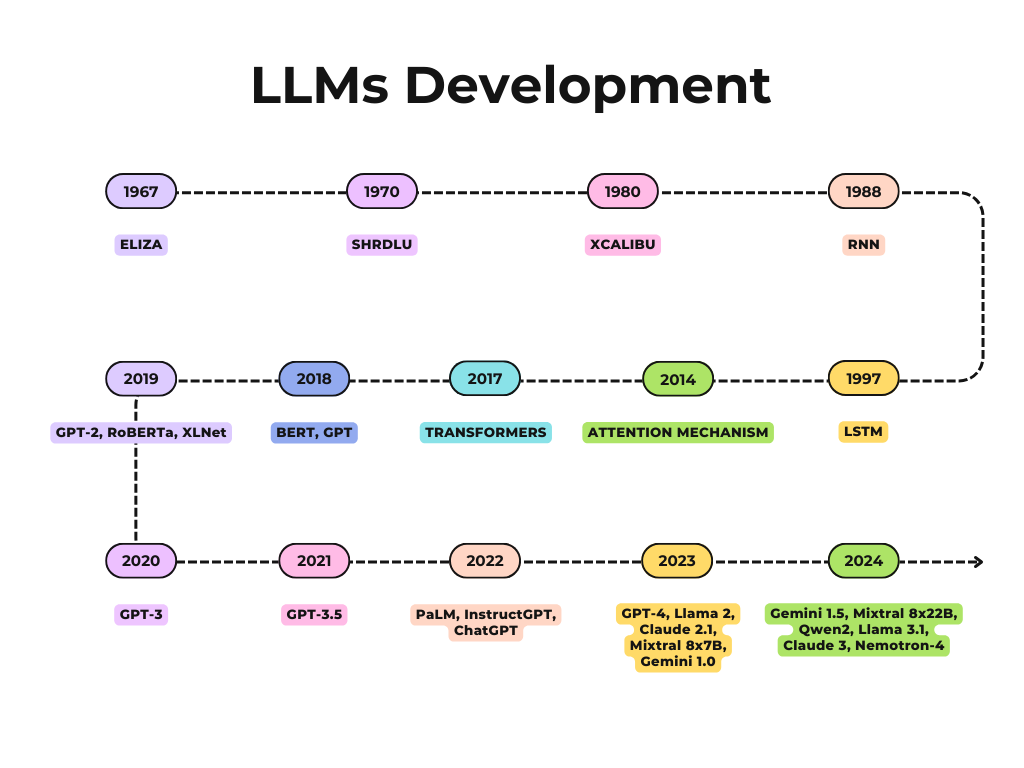
\includegraphics[width=0.9\textwidth]{images/llms/llms-timeline.png}
    \caption{Timeline of Large Language Models (LLMs) development.}
    \label{fig:llms-history}
\end{figure}

\subsubsection{Rise of Recurrent Neural Networks (1980s)}

Recurrent neural networks (RNNs), inspired by the interconnected neurons of the human brain, were developed in the late 20th century. Introduced in 1986, RNNs gained popularity due to their ability to retain previous inputs and process sequential data, making them suitable for NLP tasks. However, RNNs have shown limitations in processing long sentences, often encountering the vanishing gradient problem \cite{elman1990finding}.

\subsubsection{Rise of Long Short-Term Memory (1990s)}

In 1997, long short-term memory (LSTM), a specialized type of RNN, was introduced to address the limitations of RNNs. LSTMs are able to retain information for prolonged sequences, thus overcoming the short-term memory limitations of RNNs. The unique architectural configuration of LSTMs, which includes input, forgetting and output gates, enables them to retain relevant information within the memory system, thus improving the efficiency of capturing long-term dependencies in sentences \cite{hochreiter1997long}.

\subsubsection{Gated Recurrent Units (2010s)}

In 2014, Gated Recurrent Units (GRUs) were introduced, a means of addressing similar problems to those encountered with LSTM units, but with a simpler architectural configuration. GRUs use a simpler approach, comprising only two ports: an update gate and a reset gate. This architectural simplicity allows for greater computational efficiency while preserving the long-term dependencies inherent in the sentences \cite{cho2014learning}.

\subsubsection{Rise of Attention Mechanism (2014)}

The introduction of the attention mechanism in neural machine translation in 2014 marked a paradigm shift in sequence modeling. Unlike RNNs, which process sentences with a context vector of fixed size, attention mechanisms allowed models to dynamically select relevant parts of the source sequence, thus avoiding the loss of crucial information, especially in longer sequences \cite{bahdanau2014neural}.

\subsubsection{The Invention of Transformers Architecture (2017)}

In their 2017 paper, "Attention is All You Need", Vaswani et al. \cite{vaswani2017attention} revolutionized sequence modeling by introducing the Transformers architecture, which fundamentally shifted the field by leveraging an attention mechanism to process sequences with unprecedented efficiency and flexibility. The processors were built with an encoder-decoder architecture that includes multiple levels of self-attention and feed-forward neural networks. The multilevel attention mechanism allowed the processors to simultaneously focus on different elements of the input sentence, thus capturing a multitude of contextual subtleties. In addition, processors were able to process sequences in parallel, rather than sequentially. This paved the way for the development of sophisticated LLMs, such as BERT and GPT. Given the central role and pervasive impact of transformer architecture in the field of artificial intelligence, a fuller examination of this topic will be undertaken in subsequent sections.

\subsubsection{Emergence of Large Language Models (2018-Onwards)}

In light of the remarkable success of Transformers, it became evident that scaling these models was a logical next step. Google's BERT model, released in 2018, processed text bidirectionally, thereby setting new performance standards in a number of benchmarks \cite{devlin2018bert}. The release of OpenAI's GPT-2 in 2019 and GPT-3 in 2020 demonstrated the capabilities of generative models in performing a wide range of tasks \cite{radford2019language}. OpenAI continued to further develop the GPT series with the introduction of GPT-3.5 in 2022, GPT-4 in 2023, and GPT-4o in 2024. After its release in November 2022, ChatGPT, which is based on GPT-3.5, became the fastest growing consumer application in history.

In addition, other prominent entities in the technology industry and academia have contributed significantly to the progress of LLMs. In March 2023, Google released PaLM (Pathways Language Model), followed by the release of PaLM 2 in May 2023 \cite{chowdhery2023palm}. In December 2023, Google revealed Gemini, a multimodal model capable of processing different forms of information \cite{team2023gemini}. In 2023, Meta AI released the LLaMA (Large Language Model Meta AI) series, which offers open-source models for research and commercial use \cite{touvron2023llama}. In the same year, Anthropic introduced the Claude series, focusing on the universal benefits and security of AI \cite{anthropic2024claude}.

The advancement of language models from initial rule-based structures to current sophisticated forms represents a substantial step forward in the field of artificial intelligence. Currently, LLMs are not only tools for improving text-based applications, but are progressively demonstrating the ability to understand and interact with humans. Moreover, multimodal LLMs are able to handle not only text, but also images, sounds and videos, integrating different forms of data to comprehensively understand and analyze different contexts. These models are transforming the way humans interact with technology, making it more accessible and responsive to human needs. In essence, LLMs are becoming valuable partners for humans, assisting us in completing numerous tasks and simplifying our daily lives in many ways \cite{researchgraph2024}.

To fully understand the impact and capabilities of modern LLMs, it is essential to understand the underlying architecture that powers them. The advent of the Transformer architecture was a pivotal moment in the evolution of these models, providing the foundation for their remarkable advancement and wide applicability.

\section{The Transformer Architecture}

As mentioned in the previous section, pivotal breakthrough in the evolution of LLMs was the introduction of the Transformer architecture in 2017, as detailed in the seminal paper by Vaswani et al. \cite{vaswani2017attention}. This architecture, along with the self-attention mechanism, has since become central to all modern state-of-the-art LLMs, revolutionizing the field of natural language processing (NLP) by enabling models to capture long-range dependencies with far greater efficiency than previous architectures allowed.

\begin{figure}[h!]
    \centering
    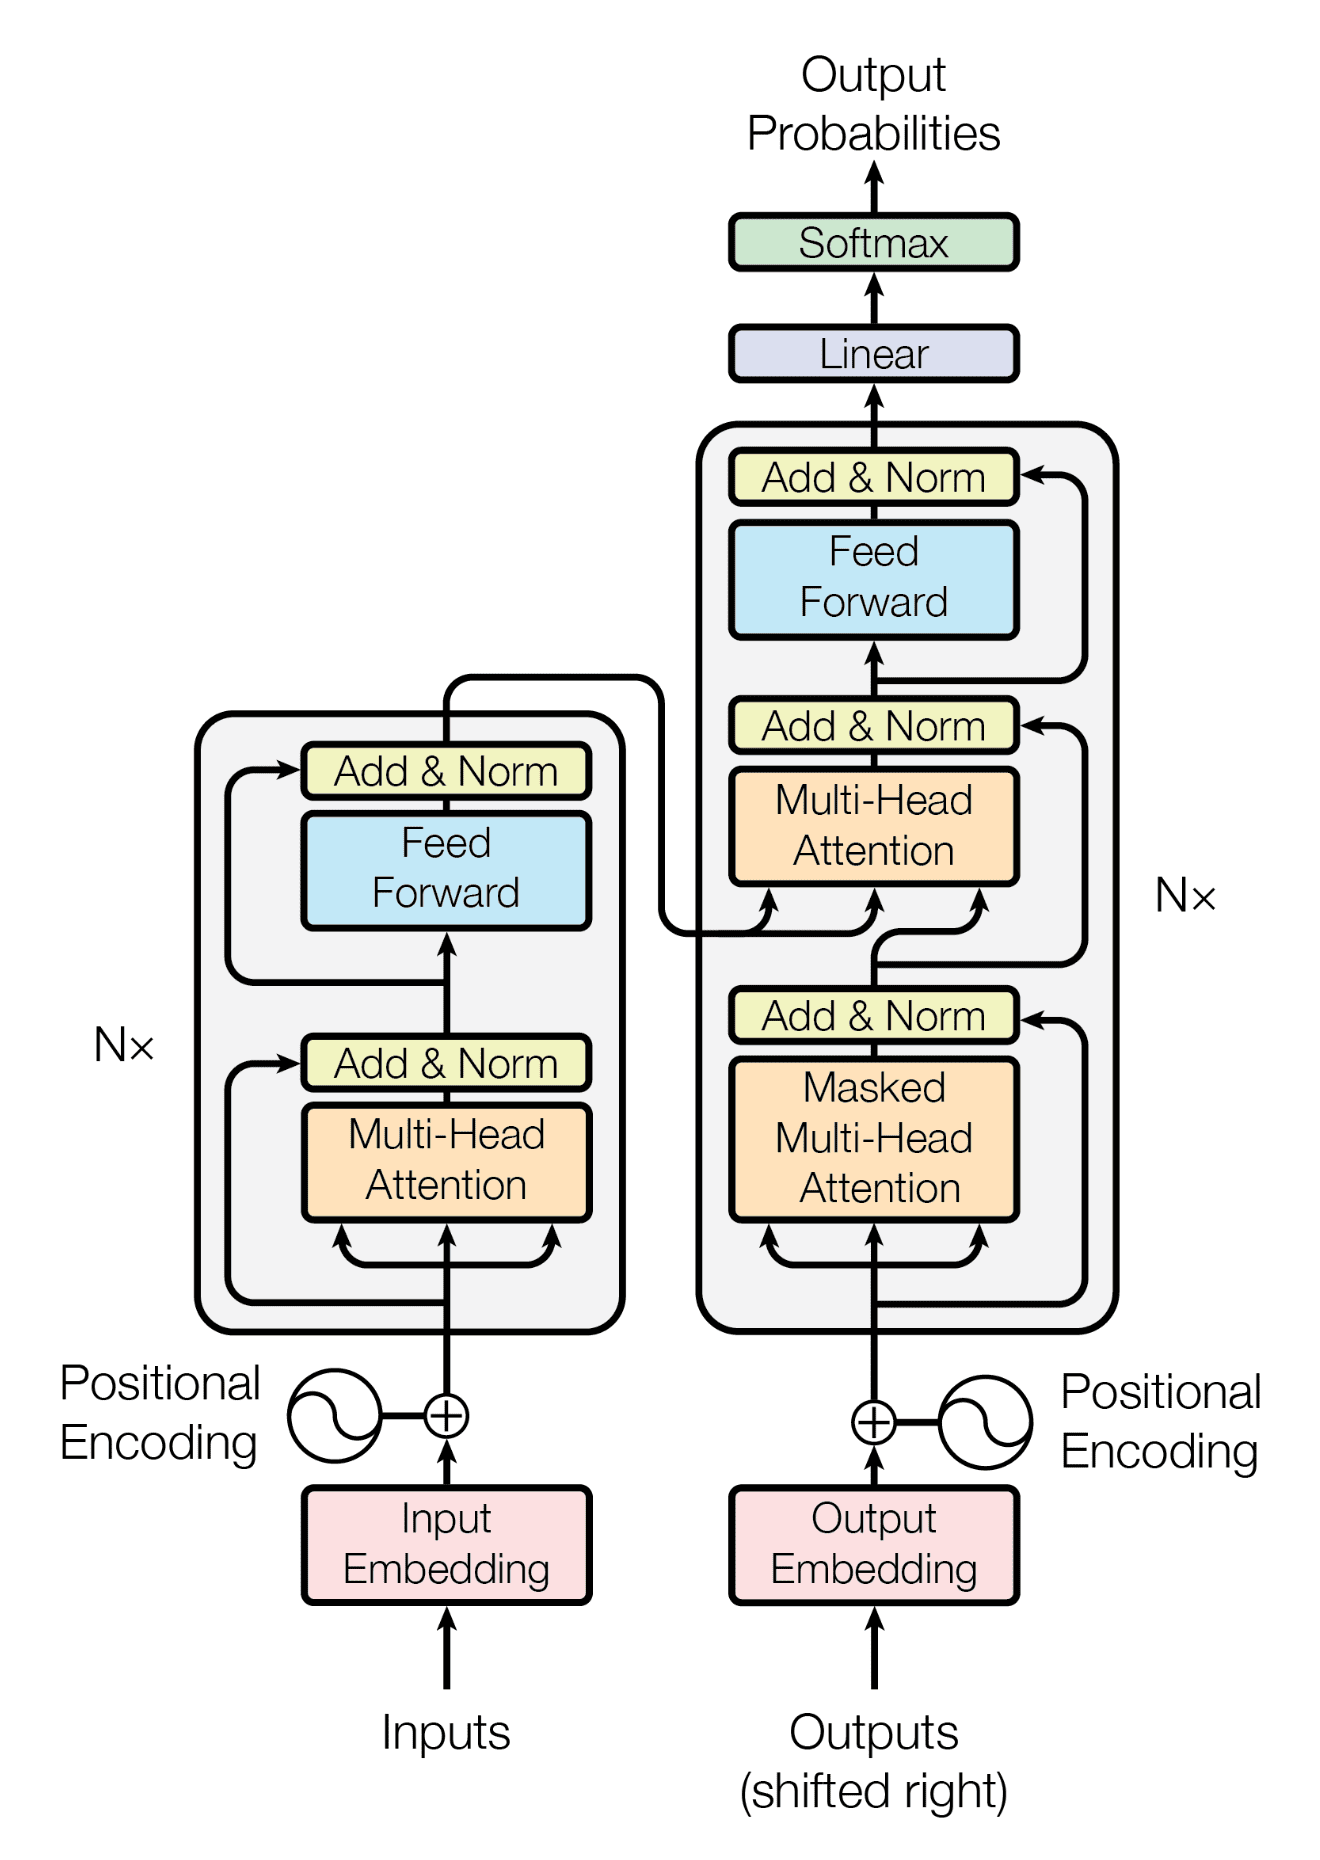
\includegraphics[width=0.6\textwidth]{images/llms/transformer-architecture.png}
    \caption{The general architecture of the Transformer, composed of an encoder and a decoder. The encoder processes the input sequence into continuous representations, while the decoder generates the output sequence from these representations. \textit{Source:} \cite{vaswani2017attention}}
    \label{fig:transformer-architecture}
\end{figure}

At the heart of the Transformer architecture is the self-attention mechanism, which enables the model to assess the relative importance of different elements within a sequence. This mechanism performs a similarity calculation between elements, thus allowing each element to direct its attention to others as needed. As a result, the model is able to understand complex relationships and dependencies in the entire input sequence, greatly enhancing its ability to generate consistent and contextually appropriate outputs. In the field of NLP, this self-attention mechanism is particularly effective in modeling the relationships between words in a sentence, thereby improving the model's ability to understand and generate nuanced, context-aware text.

One of the strengths of the Transformer architecture is its high degree of parallelization, which contributes to its computational efficiency and its ability to handle input sequences of varying lengths. Unlike traditional architectures, which process sequences sequentially, Transformers process all elements simultaneously. The Transformer's parallel processing capability greatly reduces training time, particularly for large datasets. This makes the Transformer the basis for state-of-the-art models in machine translation, text generation and numerous other NLP tasks.

As shown in Figure \ref{fig:transformer-architecture}, the Transformer architecture is composed of two main components: an encoder and a decoder. The encoder converts the input sequence into continuous representations, while the decoder generates the output sequence from these representations. The following sections will delve deeper into the key components of the Transformer, including positional encoding, multi-head attention, feed-forward neural networks, and other elements that contribute to its powerful performance in NLP and AI.

\subsection{Positional Encoding}

Unlike traditional recurrent neural networks (RNNs) and convolutional neural networks (CNNs), transformers process tokens in parallel and have no intrinsic understanding of the sequence of tokens. The incorporation of positional encodings is a key technique for integrating transformer models with sequence order understanding, thus facilitating efficient processing and understanding of input sequences \cite{li2023transformer}.

Positional encoding plays a key role in transformer models for several reasons:

\begin{itemize}
    \item \textbf{Preserve sequence order:} Transformers process tokens in parallel and have no intrinsic knowledge of the sequence of tokens. The use of positional encodings allows the model to discern between tokens based on their respective positions. This is critical for tasks where word order is a significant factor, such as language translation and text generation.
    
    \item \textbf{Maintaining Contextual Information:} In the context of NLP tasks, the interpretation of a word often depends on its position within the sentence. For example, the word "cat" in the sentence "The cat sat on the carpet" has a different meaning than the sentence "The carpet sat on the cat". The use of positional encodings serves to facilitate the retention of contextual information by allowing the model to ascertain the precise meaning based on the sequence of words.
    
    \item \textbf{Improving generalization:} The incorporation of positional information allows transformer models to generalize better between sequences of different lengths. This is especially important for tasks where the length of the input sequence is variable, such as summarizing documents or question answering. Using positional encoding allows the model to process input sequences of different lengths without any decrease in performance.
    
    \item \textbf{Mitigate symmetry:} In the absence of positional encoding, the self-attention mechanism of transformational models treats tokens symmetrically, which can lead to the generation of ambiguous representations. The introduction of positional encoding introduces asymmetry, whereby tokens in different positions are treated distinctly. This improves the ability of the model to capture long-range dependencies \cite{geeksforgeeks2024-pe}.
\end{itemize}

These enhancements not only allow the model to generalize more effectively across sequences of varying lengths but also address the inherent symmetry problem in self-attention mechanisms.

The original Transformer paper by Vaswani et al. \cite{vaswani2017attention} introduced sinusoidal positional encodings to incorporate positional information into token embeddings. This enables the model to distinguish the position of each token within a sequence. For position \( p \) and dimension \( i \), the positional encoding is calculated as:

\begin{equation}
    PE(p, 2i) = \sin\left(\frac{p}{10000^{2i/d}}\right)
\end{equation}

\begin{equation}
PE(p, 2i + 1) = \cos\left(\frac{p}{10000^{2i/d}}\right)
\end{equation}

where \( d \) is the dimensionality of the embeddings. These sinusoidal functions provide unique positional encodings that can be used by the attention mechanism to understand token order. Each dimension of the positional encoding corresponds to a sine or cosine function with a different wavelength, creating a range of frequencies from \( 2\pi \) to \( 10000 \times 2\pi \). This allows the model to capture relative positions between tokens in a sequence effectively \cite{vaswani2017attention}.


Kazemnejad \cite{kazemnejad2019:pencoding} emphasizes the ability of this encoding scheme to capture positional information in a way that satisfies several important criteria: it must produce a unique encoding for each time step, maintain consistent distances between time steps in sentences of different lengths, generalize to longer sentences, and remain deterministic.

In more recent LLMs, positional encoding often uses learned encodings rather than sinusoidal encodings. In this approach, positional encodings are randomly initialized model parameters learned during training, similar to token encodings. The size of the learned positional encoding vector is related to the maximum sequence length that the model can handle. Although the fixed maximum input length is a disadvantage of learned positional encodings, they can adapt during training, allowing the model to learn positional representations better suited to the training data, unlike static sinusoidal encodings. These advancements in positional encoding are foundational to the ability of transformers to understand the order of tokens in a sequence, but they work hand-in-hand with another crucial element: the self-attention mechanism.


\subsection{Self-attention mechanism}

The self-attention mechanism is a fundamental component of Transformer architecture, allowing the model to dynamically determine the relative importance of different words within a sequence. This capability is crucial for capturing context and understanding relationships between words, which significantly enhances the model's ability to learn long-range dependencies and generate coherent, context-aware outputs. Unlike previous architectures that struggled with processing long sequences, the self-attention mechanism allows each token in a sequence to consider the entire sequence, thereby enabling a more integrated understanding of context across tasks like translation, summarization, and question answering \cite{vaswani2017attention}.

In the self-attention mechanism, each token in an input sequence \( X \), consisting of tokens \( x_1, x_2, \ldots, x_n \), is mapped to three vectors:

\begin{itemize}
    \item \textbf{Query (Q):} Represents the focus of the model at a specific token.
    \item \textbf{Key (K):} Represents all tokens in the sequence that the query will be compared against.
    \item \textbf{Value (V):} Contains the actual information that could be relevant to the query.
\end{itemize}

These vectors are derived from the embeddings of the input tokens via learned weight matrices \( W_Q \), \( W_K \), and \( W_V \). The self-attention mechanism processes each token through the following steps:

\begin{enumerate}
    \item \textbf{Compute attention scores:} The Query vector of the current token is multiplied by the Key vectors of all tokens in the sequence, yielding attention scores that indicate the relevance of each token to the query.

    \begin{equation}
        \text{score}(Q, K) = Q \cdot K^T
    \end{equation}
    
    \item \textbf{Apply Softmax normalization:} These attention scores are then normalized using a softmax function, which converts them into a probability distribution, ensuring that the sum of the attention weights across all tokens is equal to 1. This process usually involves scaling by the square root of the Key vector's dimensionality, \( \sqrt{d_k} \), to maintain numerical stability.

    \begin{equation}
        \text{Attention}(Q, K) = \text{softmax}\left(\frac{Q \cdot K^T}{\sqrt{d_k}} \right)
    \end{equation}
    
    \item \textbf{Generate the output:} The resulting attention weights are then used to compute a weighted sum of the Value vectors, which produces the final output for the token. This output is a contextually enriched representation that captures the relationships and dependencies within the sequence \cite{vaswani2017attention}.

    \begin{equation}
        \text{Output} = \text{Attention}(Q, K) \cdot V
    \end{equation}
\end{enumerate}

Through this mechanism, the Transformer can effectively focus on the most relevant parts of the input sequence, enabling a comprehensive understanding of complex dependencies and improving the model's overall performance in generating accurate and contextually appropriate responses. The self-attention mechanism's ability to integrate and contextualize information from across the entire sequence is a key factor in the success of Transformer-based models \cite{geeksforgeeks2024-sa}.

Building on this foundational concept, the Transformer architecture further refines its attention capabilities through the use of multi-head attention, which allows the model to capture multiple aspects of the input data simultaneously and enhances its ability to understand complex patterns and relationships.

\subsection{Multi-Head Attention}

The multi-head attention mechanism builds upon the basic self-attention mechanism, significantly enhancing the model's ability to capture various aspects of the input data. Instead of relying on a single execution of self-attention, the transformer applies this operation multiple times in parallel, each time using a different set of learned weight matrices. This parallelism allows the model to learn and represent different features of the input data simultaneously, providing a richer and more diverse understanding of the input sequence.

In multi-head attention, there are \( h \) distinct sets of weight matrices: \( W_Q \), \( W_K \), and \( W_V \). Each head independently performs the self-attention operation and produces its output. The results from all heads are then concatenated and passed through a final linear transformation using a learned weight matrix \( W_O \) to generate the final output of the multi-head attention layer:

\begin{equation}
    \textit{MultiHeadOutput} = \textit{Concat}(\textit{head}_1, \textit{head}_2, \ldots, \textit{head}_h) \cdot W_O
\end{equation}

This approach allows each attention head to focus on different aspects or relationships within the input data. For instance, when processing a sentence, one head might focus on syntactic structures, another on semantic meaning, and yet another on sentiment or tone. The combination of these different perspectives leads to a more comprehensive and nuanced representation of the input sequence.

The advantage of multi-head attention lies in its ability to capture a broader range of relationships and interactions within the data, which is crucial for generating more accurate and contextually appropriate outputs. This capability makes the transformer architecture, and by extension, multi-head attention, particularly powerful for natural language processing (NLP) tasks such as translation, summarization, and text generation \cite{geeksforgeeks2024-sa}.

\begin{equation}
    \textit{MultiHead(Q, K, V)} = \textot{Concat}(\textit{head}_1, \textit{head}_2, \ldots, \textit{head}_h) \cdot W_O
\end{equation}

By enabling the model to attend to different parts of the input sequence simultaneously through multiple heads, the multi-head attention mechanism is a crucial component of the transformer architecture. It plays a key role in advancing the state-of-the-art in NLP, contributing to the development of sophisticated language models that excel in a wide range of applications \cite{vaswani2017attention}.

\subsection{Feed-Forward Neural Networks}

In the transformer architecture, after processing of the input sequence by the multi-headed attention mechanism, each position in the sequence is passed independently through a feed-forward neural network (FFNN). The network is identical for each position, with the same weights and biases applied to all inputs, regardless of their position within the sequence.

The FFNN comprises two linear transformations, with a ReLU (Rectified Linear Unit) activation function applied between them:

\begin{itemize}
    \item \textbf{First Linear Transformation}: The initial step involves multiplying the input by a weight matrix \( W_1 \) and adding a bias \( b_1 \), resulting in a transformed version of the input data.
    \item \textbf{ReLU Activation Function}: The transformed input then passes through a ReLU activation function, which introduces non-linearity into the model, enabling it to capture complex patterns within the data. The ReLU function is mathematically defined as:
    \begin{equation}
        \text{ReLU}(x) = \max(0, x)
    \end{equation}
    \item \textbf{Second Linear Transformation}: After the ReLU activation, the output is passed through a second linear transformation, where it is multiplied by another weight matrix \( W_2 \) and a bias \( b_2 \) is added, producing the final output of the FFNN.
\end{itemize}

The entire process of the FFNN, given an input \( x \), can be summarized by the following equation:
\begin{equation}
    \text{FFN}(x) = \text{ReLU}(x \cdot W_1 + b_1) \cdot W_2 + b_2
\end{equation}

Where:
\begin{itemize}
    \item \( x \) represents the input to the FFNN.
    \item \( W_1 \) and \( W_2 \) are the weight matrices for the first and second linear transformations, respectively.
    \item \( b_1 \) and \( b_2 \) are the corresponding bias vectors.
\end{itemize}

All of these parameters—\( W_1 \), \( W_2 \), \( b_1 \), and \( b_2 \)—are learnable and are optimized during the training process.

The multi-headed attention mechanism allows the Transformer model to focus on different elements of the input sequence, while the FFNN applies further transformation to the attention output. This combination of attention and feed-forward processes enables the Transformer to perform effectively across a wide range of sequence transduction tasks, such as text generation, named entity recognition, and question answering, by providing an additional layer of abstraction and data transformation \cite{vaswani2017attention}.

\subsection{Stabilizing Transformer Layers: Add \& Norm Step}

After the input processing by the multi-headed attention mechanism and feed-forward neural network layer in the transformer architecture, the output is stabilized through the application of the add \& norm step. This step is of great importance in maintaining the stability and efficiency of the model during training, enabling the architecture to support the deep, multilayer structures common in advanced models. The add \& norm step consists of two main components: residual connection and layer normalization.

\subsubsection{Residual Connections for Enhanced Stability (Add)}

Residual connections, also known as "skip connections," serve as a shortcut by adding the input of a sublayer directly to its output. This mechanism allows the network to effectively learn identity mappings when the optimal action for a particular layer is to leave the input largely unchanged. In such cases, the weights of the sublayer can be minimized to near zero, making its output negligible (\(\text{SubLayer}(X) \approx 0\)). By adding this output to the original input \(X\) through the residual connection, the resultant output closely approximates \(X\), effectively preserving the original input. This identity mapping not only enhances model performance but also significantly stabilizes the training process. The operation is mathematically expressed as:

\begin{equation}
    Z = X + \text{SubLayer}(X)
\end{equation}

Where:
\begin{itemize}
    \item \(X\) represents the input to the sublayer.
    \item \(\text{SubLayer}(X)\) denotes the transformations applied by the sublayer to \(X\).
    \item \(Z\) is the output after the residual connection is applied.
\end{itemize}

Residual connections are crucial for mitigating the vanishing gradient problem, a common issue in deep neural networks with many layers. As gradients are backpropagated, they may diminish, leading to minimal updates in the early layers, which can hinder or completely stop learning. By allowing gradients to bypass the sublayer via the addition operation, residual connections ensure that substantial gradients reach the earlier layers, thereby addressing the vanishing gradient issue and facilitating the training of deep networks.

\subsubsection{Layer Normalization for Stable Activation Scaling (Norm)}

After applying residual connections, the Transformer model utilizes layer normalization to standardize the activations for each feature as they move through the multi-head attention and feed-forward network layers. This normalization technique adjusts the activations based on their computed mean and variance, ensuring they are rescaled to have a mean of zero and a unit variance, regardless of the input or the layer within the Transformer.

Given an input \( Z \) to the layer normalization, the mean \( \mu_Z \) and variance \( \sigma_Z^2 \) are calculated as:

\begin{equation}
\mu_Z = \frac{1}{d} \sum_{i=1}^{d} Z_i \quad \text{and} \quad \sigma_Z^2 = \frac{1}{d} \sum_{i=1}^{d} (Z_i - \mu_Z)^2
\end{equation}

where \( d \) is the dimension of the feature vector \( Z \). The normalized value \( \hat{Z}_i \) for each feature is then derived by:

\begin{equation}
\hat{Z}_i = \frac{Z_i - \mu_Z}{\sqrt{\sigma_Z^2 + \epsilon}}
\end{equation}

Here, \( \epsilon \) is a small constant included for numerical stability. Once the normalization is complete, the activations are further adjusted by applying learnable scaling and shifting parameters:

\begin{equation}
\text{Norm}(Z)_i = \gamma \hat{Z}_i + \beta
\end{equation}

where \( \gamma \) and \( \beta \) are the learnable parameters that scale and shift the normalized activations, respectively, with dimensions corresponding to those of \( Z \).

Layer normalization ensures that the activations remain consistent in scale across different layers, thereby preventing gradients from either diminishing or exploding as they propagate through the model. This, in combination with residual connections, effectively addresses the vanishing and exploding gradient issues, facilitating the training of deep Transformer architectures.

Together, these mechanisms contribute to the robust performance of the Transformer, allowing it to effectively manage deep networks and maintain stable learning.

\subsection{Encoder and Decoder Stacks}

The transformer architecture consists of a series of encoding and decoding blocks, arranged in a stack configuration. Each block consists of both multi-headed attention layers and feedforward neural network layers. Stacking multiple blocks allows for increased representation power, enabling the model to learn complex patterns and relationships within the data.

The transforming encoder is responsible for processing the input sequence and transforming it into a series of continuous representations. Each layer of the encoder employs a multi-headed self-attention mechanism, followed by a fully connected position-based feed-forward network. This architecture allows the encoder to effectively capture and understand the different elements of the input sequence.

The decoder, on the other hand, is responsible for generating the output sequence, using the continuous representations provided by the encoder. Similarly, each layer of the decoder is composed of a multi-headed self-attention mechanism and a feed-forward network, similar to those in the encoder. In addition, the decoder incorporates an attention mechanism between the encoder and the decoder, which allows it to focus on relevant aspects of the input sequence during output generation. This attention mechanism ensures that the generated sequence is contextually consistent with the input sequence \cite{vaswani2017attention}.

\subsection{Final Linear and Softmax Layer}

The decoder output goes through a final linear layer and then a softmax layer to create a probability distribution over the target vocabulary. In the context of an NLP task using a transformer model, the target vocabulary includes all possible words, tokens, or symbols that the model can generate \cite{jozefowicz2016exploring}. The linear layer converts the high-dimensional representations produced by the decoding stack to a dimensionality that corresponds to the size of the target vocabulary. Next, the softmax function is applied to these raw scores, converting them into probabilities such that the total probability of all vocabulary tokens is equal to one. The resulting probability distribution reflects the model's prediction of the probability that each target vocabulary token is the next token in the sequence, thus enabling operations such as translation and text generation.

These final layers are crucial for transforming the abstract representations learned by the Transformer into actionable outputs, ultimately enabling the model to perform complex tasks such as language translation, summarization, and text generation. By synthesizing the outputs of the preceding layers into a coherent probability distribution, the final linear and softmax layers encapsulate the model's learned knowledge and allow it to generate meaningful and contextually appropriate sequences. This final step underscores the power of the Transformer architecture, tying together its multi-layered processing capabilities and making it one of the most effective and versatile models in modern natural language processing.

\section{Impact of Model Size on AI Performance}

The size of a neural network model, particularly in the domains of AI and NLP, is a key determinant of its performance and capabilities. The ability of a model to learn and represent complex data depends on its size, typically quantified in terms of the number of parameters. A larger model is able to encapsulate more detailed relationships, which in turn leads to greater accuracy and robustness in a variety of tasks. However, increasing model size also brings complications, including increased computational needs, increased memory usage and longer training periods.

\subsection{Evolution of Parameter Sizes in AI Neural Networks}

The progress of AI neural networks over time has been characterized by a significant increase in the number of parameters. In the early stages of AI development, models such as simple FFNNs and nascent convolutional neural networks (CNNs) had relatively small numbers of parameters. In fact, before the 2000s, language models were relatively simple and limited in scope due to computational power constraints. For example, LeNet-5, an early CNN developed by LeCun et al. \cite{lecun1998gradient} in 1998, had about 60,000 parameters. 

As computational capabilities and data availability improved, researchers were able to create larger and more complex models. In particular, the advent of deep learning and hardware advances in the 2010s led to the emergence of deeper architectures, such as VGGNet and ResNet, which significantly increased parameter sizes. For example, VGG-16 includes about 138 million parameters \cite{simonyan2014very}, while ResNet-50 has about 25 million parameters \cite{he2016deep}.

The progression to larger models has continued with the advent of transformers and LLMs. In 2018, Devlin et al. \cite{devlin2018bert} presented BERT, a transformer model with 110 million parameters in the basic version and 340 million in the larger version. OpenAI's GPT-3 (2020), with 175 billion parameters, and GPT-4 (2023), with 1.76 trillion parameters, demonstrated a significant increase in the size of LLM models, setting new benchmarks in various NLP tasks \cite{brown2020language, achiam2023gpt}.

The number of parameters in LLMs has a significant impact on their ability to discern intricate and highly dimensional relationships within data sets. In general, an increase in the number of parameters results in greater model complexity, which often leads to improved performance in a range of NLP tasks. However, larger models are more susceptible to overfitting and require significant computational resources \cite{zhao2023survey, villalobos2022machine, wei2022emergent}.

Moreover, the number of parameters in LLMs depends on the volume of data used during training. The effectiveness of complex models in capturing the intricate nuances of language depends on the availability of large and diverse textual data. The size of these training datasets is typically expressed in terms of tokens, which represent the basic units used by LLMs for text processing and generation. The specific tokenization algorithm employed can produce tokens representing a variety of linguistic units, including single characters, syllables, words or even sentence segments \cite{brown2020language}.

\subsection{Recent Trends in AI development}

The importance of model size has been further emphasized by recent developments in the field of AI, where training computation has emerged as a critical factor. Figure \ref{fig:large-scale-models} shows models with a training computation greater than 10 floating-point operations (FLOP). This threshold defines models which typically involve training costs of hundreds of thousands of dollars or more. For example, the AI Index estimates that OpenAI's GPT-4 used about \$78 million USD in computational resources for training, while Google's Gemini Ultra required an investment of \$191 million USD in computational resources \cite{epoch2024trackinglargescaleaimodels, maslej2024ai}.

\begin{figure}[h!]
    \centering
    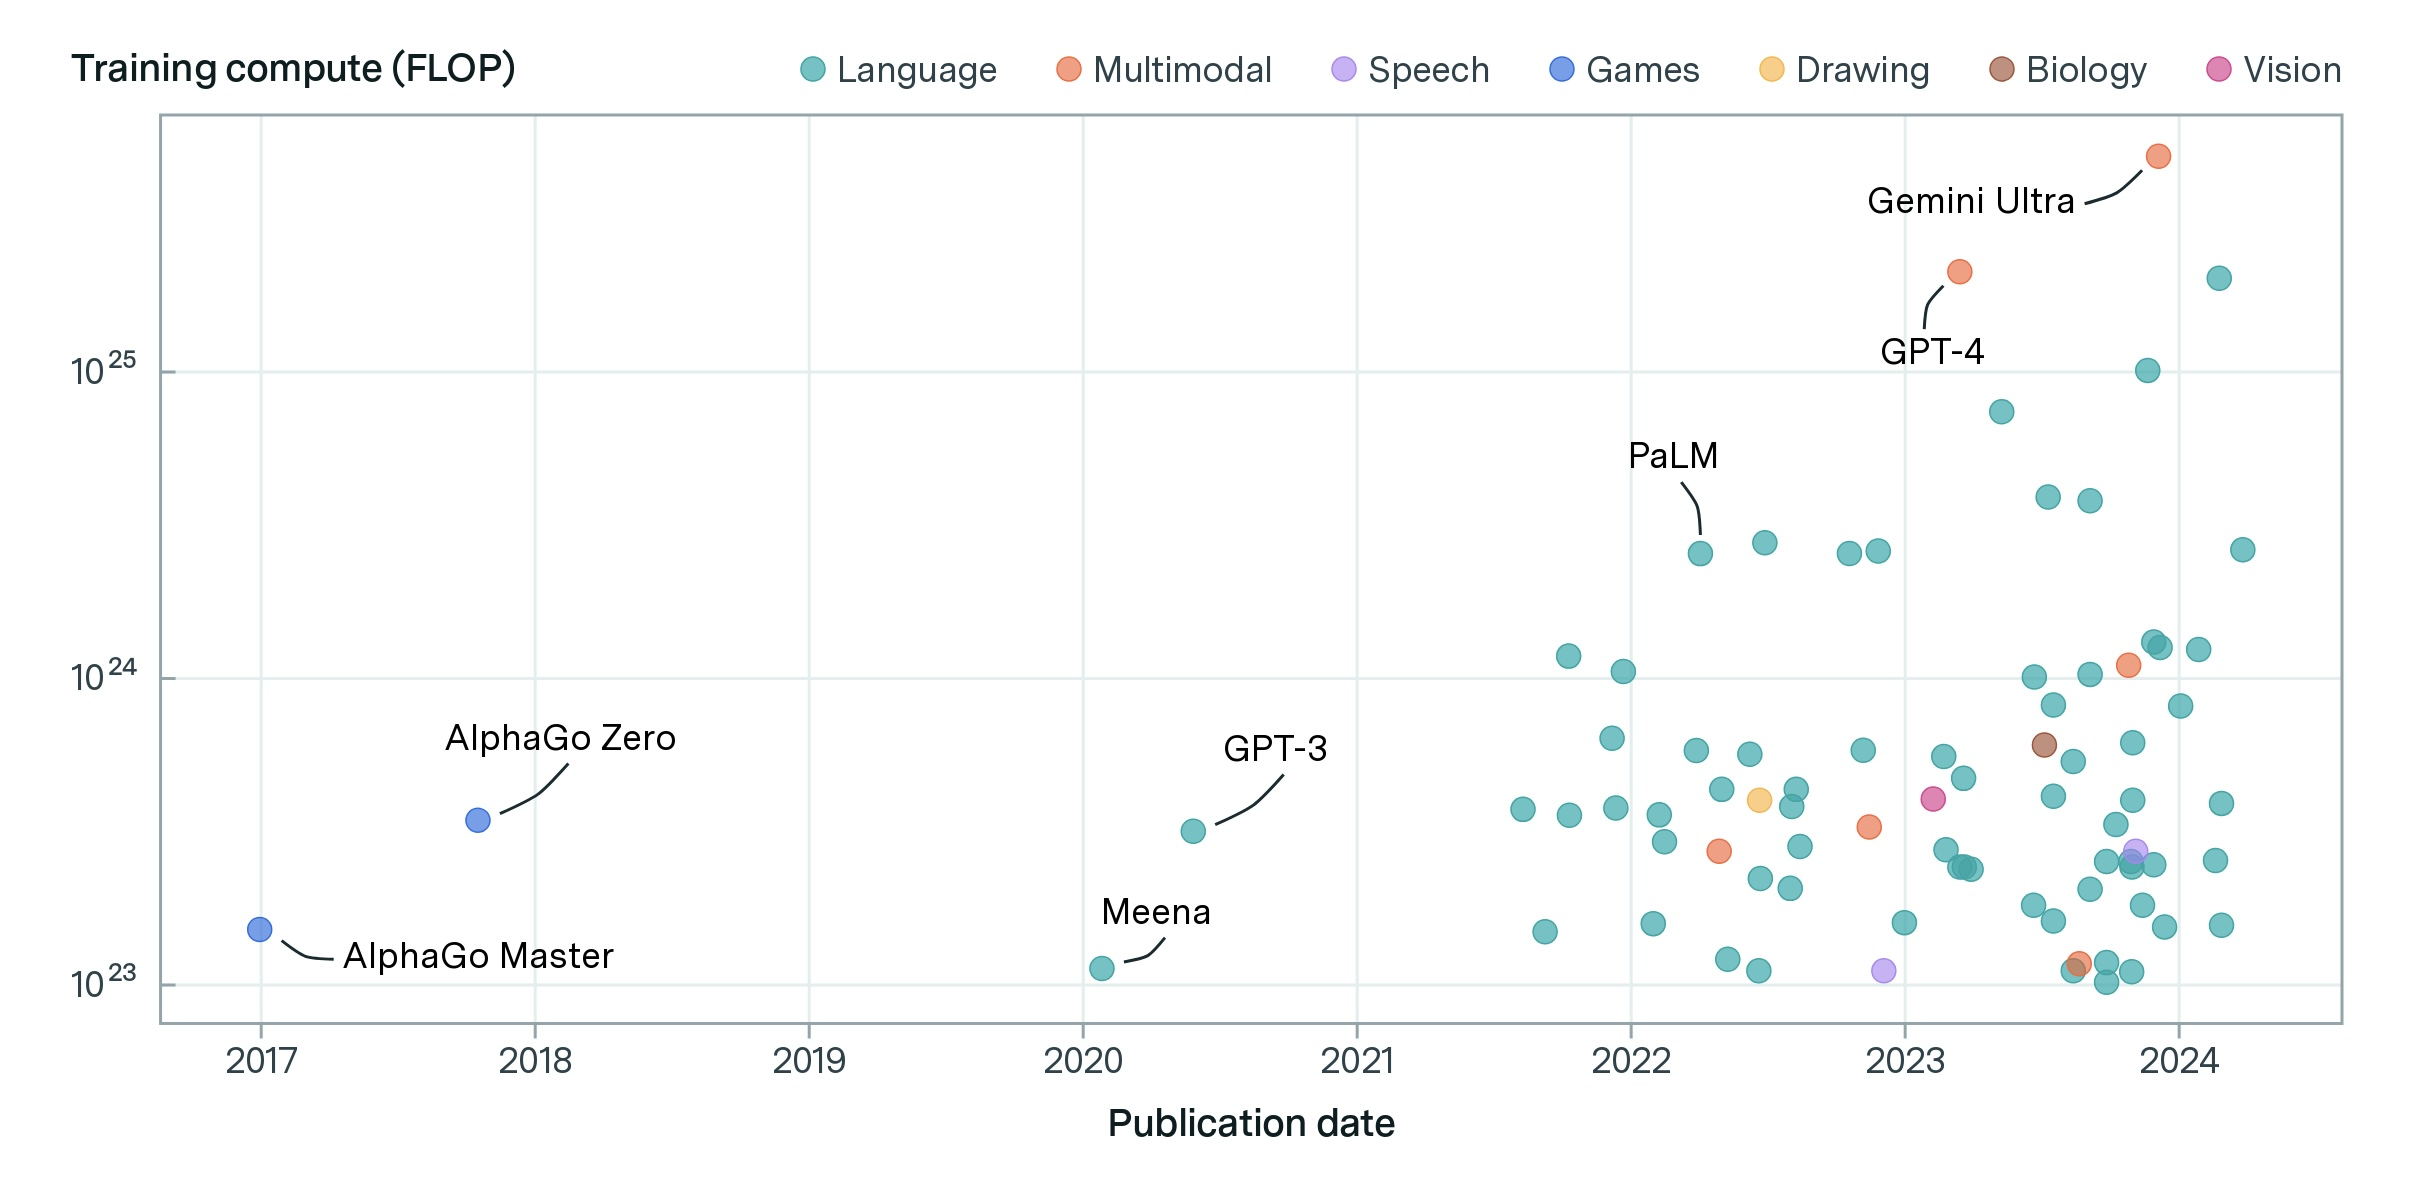
\includegraphics[width=0.9\textwidth]{images/llms/large-scale-models-by-domain-and-date.jpg}
    \caption{Large language models by domain and publication date. The graph displays the training calculation (in FLOP) of various models in different domains over time. \textit{Source:} \cite{epoch2024trackinglargescaleaimodels}}
    \label{fig:large-scale-models}
\end{figure}

In 2020, only 11 models were trained that exceeded the threshold of 10\textsuperscript{23} FLOP, but by 2024 the number had risen to 81, indicating a rapid acceleration in the release of LLMs. Most of these models are linguistic in nature, while others are multimodal or image processing models. This trend underscores the prominence of linguistic and image generation tasks in AI development from 2021 \cite{epoch2024trackinglargescaleaimodels}.

The exponential growth in research and development (R\&D) investment and hardware performance in the AI field is driving the rapid advancement of the computational frontier. Recent trends indicate a growth rate of 4-5 times per year for remarkable models between 2010 and May 2024. In the case of linguistic models, the overall growth rate has reached 9 times per year, which can be attributed to the industry's moving closer to the AI frontier. The sustained increase in training calculations highlights the need for efficient hardware and new training techniques to cope with the expansion of large-scale AI models \cite{epoch2024trainingcomputeoffrontieraimodelsgrowsby45xperyear}.

A substantial portion of LLMs have been developed in the United States, but China has also made significant contributions in recent times. The organizations that have developed the predominant LLMs are Google, Meta, DeepMind, Hugging Face and OpenAI. In addition, developers include numerous companies, academic institutions and government agencies. In the context of unconfirmed models, it is noteworthy that organizations such as Anthropic and Alibaba also occupy a prominent position. Most of the LLMs were developed by industry, while a smaller number were the result of industry-university collaborations and some were developed by government institutions. Interestingly, about half of the LLMs have downloadable and publicly available weights, which were trained primarily with calculations between 10\textsuperscript{23} and 10\textsuperscript{24} FLOP per second. However, larger proprietary models often require significantly greater computational resources and do not disclose the details of their training procedures.

Despite these considerations, the growth frontier has shown signs of deceleration, which can be attributed to prospective impediments such as data scarcity, investment propensity, data center power limits and the inability to expand chip production. These factors can have an impact on the exponential growth of computing resources needed for training advanced AI models \cite{epoch2024trainingcomputeoffrontieraimodelsgrowsby45xperyear}.

In conclusion, model size is a critical factor affecting the performance of AI neural networks. The increasing deployment of larger models has led to significant advances in AI capabilities, particularly in the field of NLP. However, it also requires a careful balance between performance and practical considerations, such as computational efficiency and resource demands. The continued increase in training computations and associated challenges underscore the need for novel approaches to ensure the continued progress of AI.

\section{Training Process}

Training LLMs is a complex process involving a series of discrete steps, each designed to improve the model's capabilities in a gradual and systematic manner. Training these sophisticated models, which include billions of parameters, has been made possible by recent advances in computing power and architectural innovations. The training process has three distinct phases: pre-training, fine-tuning, and prompt-based learning. Each stage of the training process contributes to the development and refinement of the model in a particular way (see Figure \ref{fig:training-process}).

LLMs undergo an initial pre-training phase, during which the model is trained on a substantial unlabeled dataset, which often includes a significant portion of internet text. This phase allows the LLM to develop a fundamental understanding of language structures and patterns through recognition and learning from the input data. Then, at the end of the pre-training phase, the models undergo a fine-tuning process using smaller, task-specific datasets. The goal of this tuning process is to adapt the model's capabilities to perform specialized tasks, such as translation, question answering, or chatbot functionality. The act of prompting involves engaging with an optimized model through the use of specific questions or statements, called prompts, with the goal of eliciting the desired response from the model. The following sections will examine these three essential elements of LLM training and the methodologies used to train LLMs for question-answering chatbot applications.

\begin{figure}[h!]
    \centering
    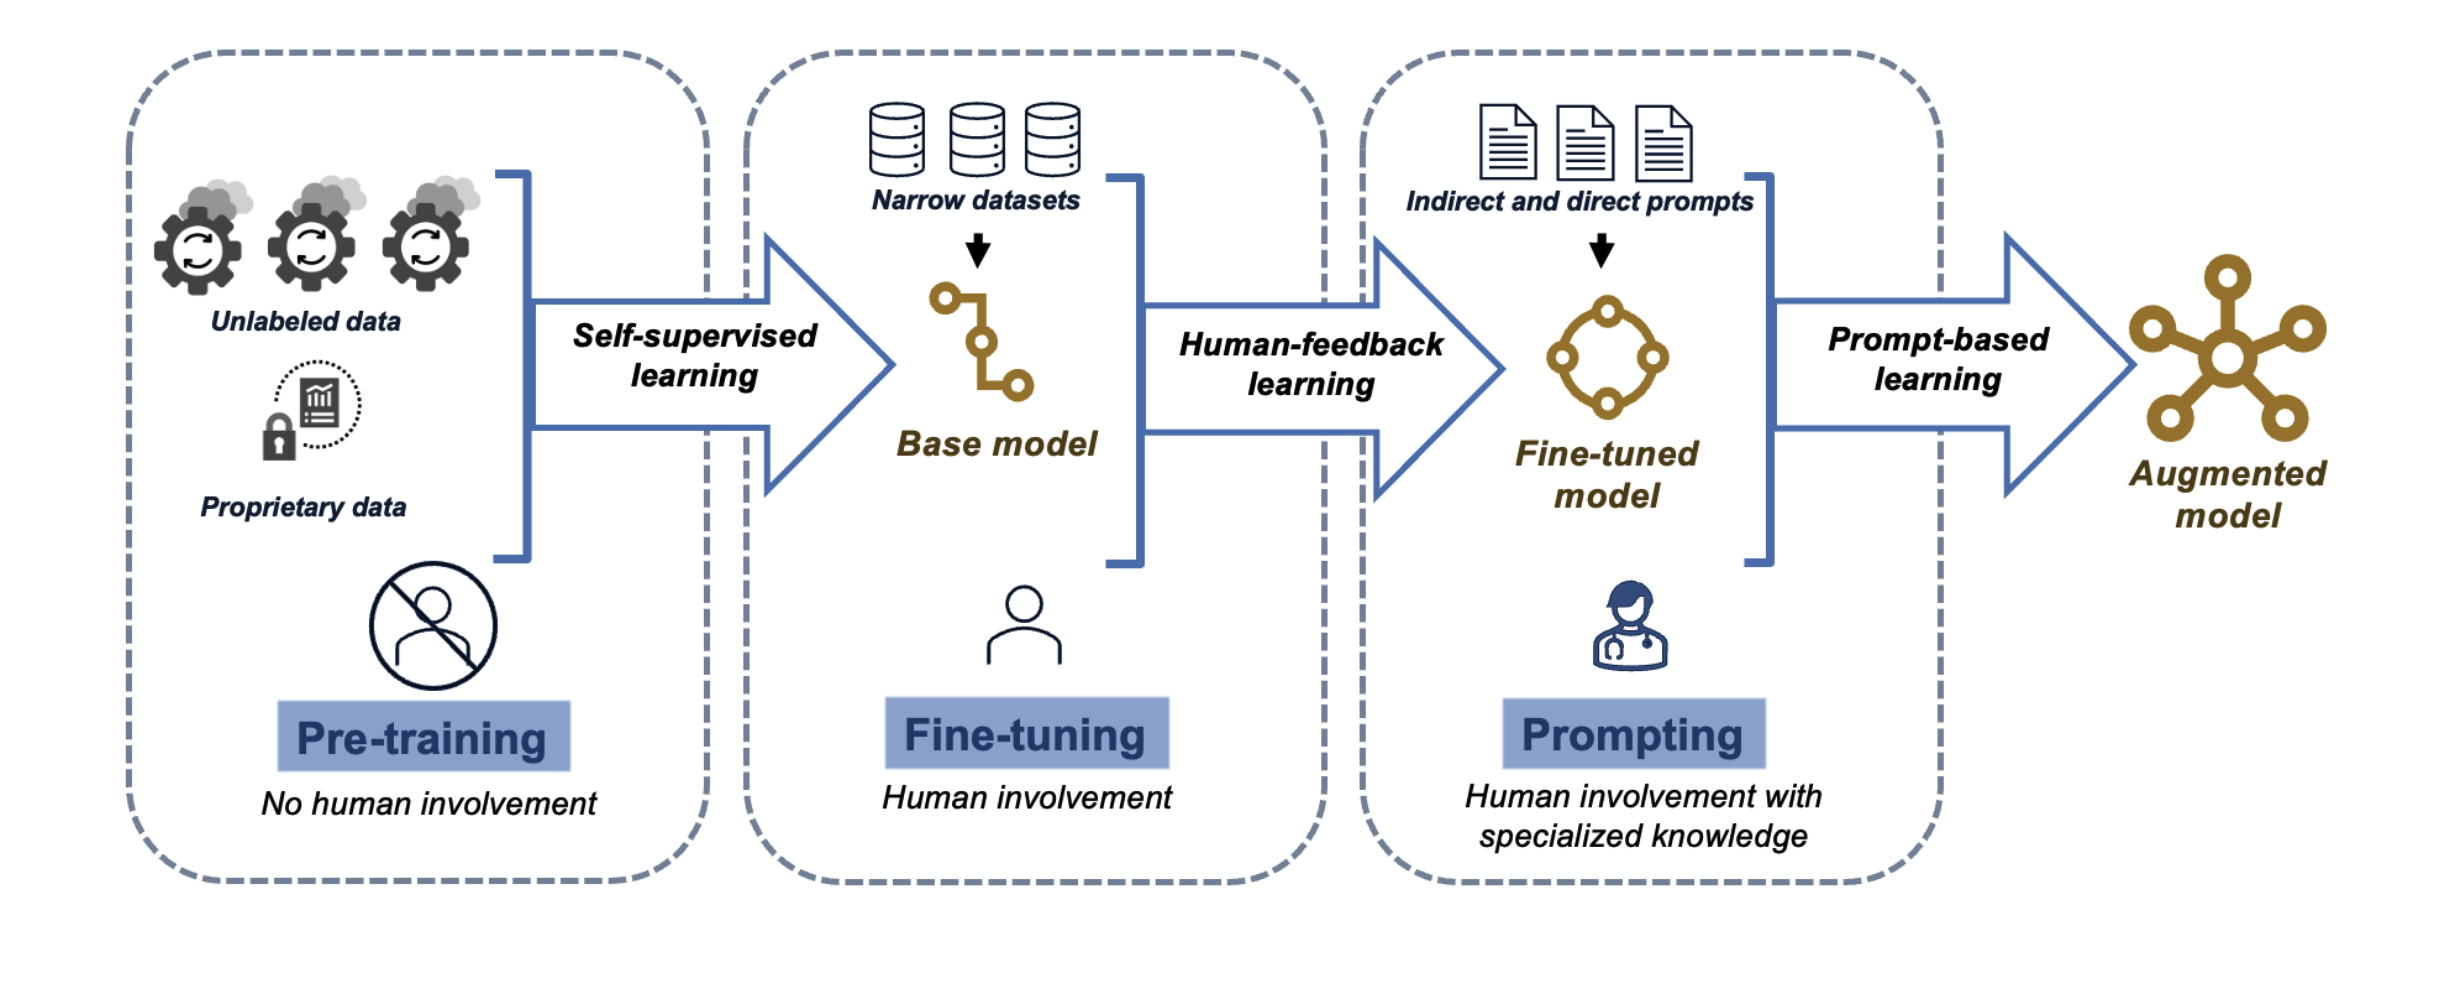
\includegraphics[width=0.9\textwidth]{images/llms/LLM-training-process.png}
    \caption{Overview of the training process of LLMs. LLMs learn from more targeted inputs at each stage of the training process. The first phase of this learning is pre-training, in which the LLM can be trained on a mix of unlabeled data without any human supervision. The second phase is fine-tuning, in which narrower data sets and human feedback are introduced as inputs to the basic model. The fine-tuned model can then enter a further phase, in which humans with specialized knowledge implement hinting techniques that can transform the LLM into an enhanced model to perform specialized tasks. \textit{Source:} \cite{omiye2023large}}
    \label{fig:training-process}
\end{figure}

\section{Pre-training}

The pre-training phase represents a crucial stage in the development of LLMs, as it facilitates their ability to understand and generate human language. This stage is a self-supervised process in which the model is trained on a substantial corpus of unlabeled data, including internet texts, Wikipedia, GitHub code, social media posts, and BooksCorpus. In addition, some models incorporate proprietary datasets that include specialized texts, such as scientific articles \cite{brown2020language, devlin2018bert}.

The main goal of the pre-training phase is to predict the next word in a sentence. This is a computationally demanding task that involves converting the text into tokens before entering them into the model. This phase produces a rudimentary model that, although capable of generating general language, lacks the sophistication needed to handle tasks that require subtlety and nuance \cite{radford2019language}.

The two principal methods for pre-training are Autoregressive Language Modeling (ALM) and Masked Language Modeling (MLM). Both approaches have had a significant impact on the development of state-of-the-art LLMs, enhancing their capacity to comprehend and produce texts that are akin to those produced by humans.

\subsection{Autoregressive Language Modeling (ALM)}

In the context of NLP, Autoregressive Language Modeling (ALM) represents a generative approach in which the model is tasked with predicting the next word in a sequence given the previous words. Autoregressive language models, exemplified by PT (Generative Pre-trained Transformer), have attracted considerable attention for their remarkable ability to generate high-quality text and perform a wide range of language-related tasks. These models use a transformer architecture to facilitate sequential processing of text data. The autoregressive mechanism enables the generation of coherent and contextually relevant texts as it samples from the probability distribution learned about vocabulary. This has been demonstrated in previous studies, including those by Radford et al. (2018, 2019) and Achiam (2023), who used GPT as a case study \cite{radford2018improving, radford2019language, achiam2023gpt}.

All the autoregressive models developed by OpenAI have used a semi-supervised learning approach, which combines elements of supervised and unsupervised learning. In particular, OpenAI introduced a methodology involving unsupervised pre-training followed by supervised tuning, which addresses the high costs associated with creating labeled datasets for language tasks.

\begin{figure}[h]
    \centering
    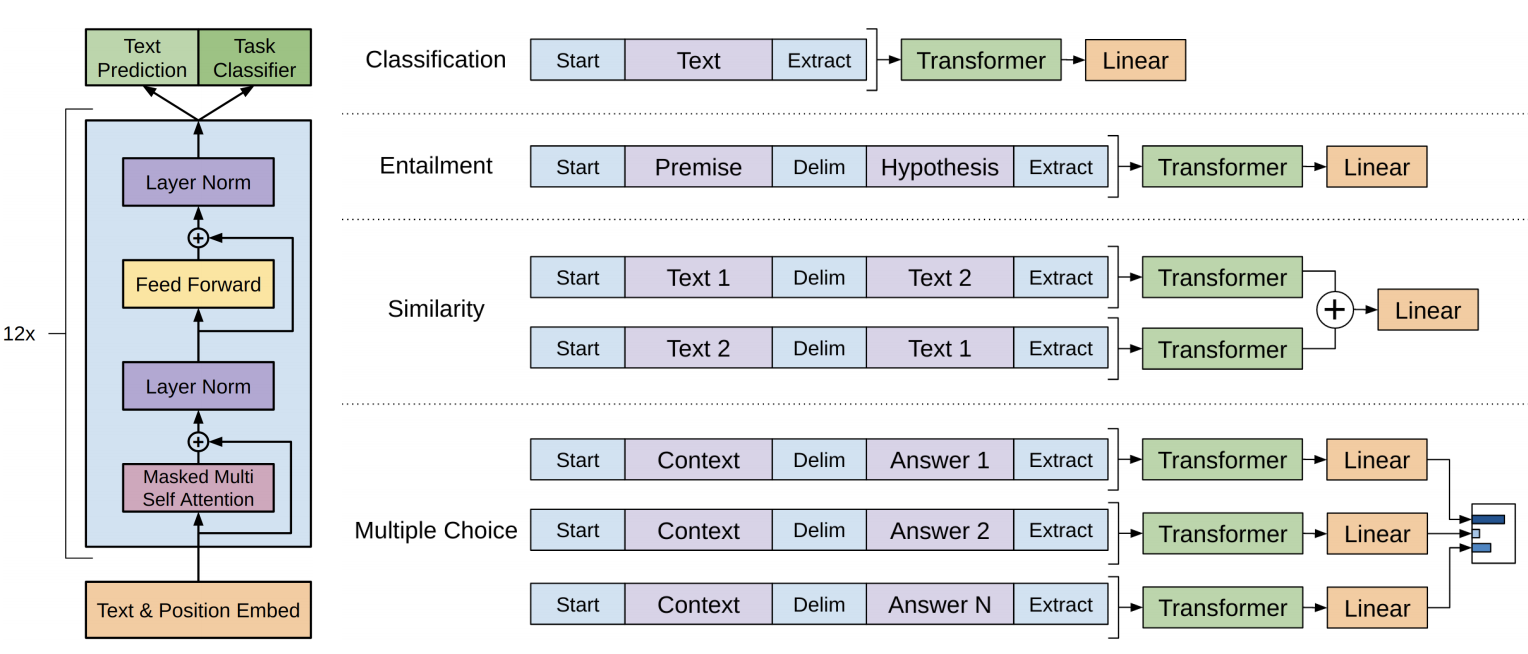
\includegraphics[width=0.9\textwidth]{images/llms/gpt.png}
    \caption{The architecture of the decoder represents the transformer of a GPT, which has been trained for the purpose of auto-regressive text generation. The diagram demonstrates the integration of text prediction and task-specific classifiers, as well as the application of multi-headed self-attention and feed-forward neural networks. \textit{Source:} \cite{radford2018improving}}
    \label{fig:transformer_architecture}
\end{figure}

In unsupervised pre-training, a high-capacity language model is trained on an extensive corpus of text with the objective of maximizing the log-likelihood of the next word given the context provided by the preceding sequence. The formal objective is stated as follows:

\begin{equation}
    \mathcal{L}_1(\mathcal{U}) = \sum_{i} \log P(u_i | u_{i-k}, \ldots, u_{i-1}; \Theta)
\end{equation}

where \( k \) represents the context window. In simpler terms, the model looks back at \( k \) tokens while predicting the \((k+1)^{th}\) token. In the pre-training phase, a multi-layer transformer decoder is utilized. Subsequently, multi-headed self-attention is applied to the input tokens, followed by a position-wise feed-forward network. The resulting output is a distribution over the target tokens.

This is subsequently followed by a supervised fine-tuning phase, where a labeled dataset with \( y \) as labels and \( x \) as inputs is utilized. The inputs are passed through the pre-trained model, and the output from the final transformer block is fed into an additional linear output layer with parameters \( W_y \) to predict \( y \). This process results in the following intermediate objective to maximize:

\begin{equation}
    \mathcal{L}_2(\mathcal{C}) = \sum_{(x,y)} \log P(y | x^1, \ldots, x^m)
\end{equation}

The incorporation of the pre-training objective as an auxiliary objective during fine-tuning has been demonstrated to enhance generalization and accelerate convergence, as evidenced by research findings \cite{radford2018improving}. Consequently, the pre-training loss \( \mathcal{L}_1 \) is integrated into the final objective with a weighting factor \( \lambda \):

\begin{equation}
    \mathcal{L}_3(\mathcal{C}) = \mathcal{L}_2(\mathcal{C}) + \lambda \ast \mathcal{L}_1(\mathcal{C})
\end{equation}
 
\subsection{Masked Language Modeling (MLM)}

In contrast, Masked Language Modeling (MLM) represents a denoising goal that is predominantly employed by models such as BERT (Bidirectional Encoder Representations from Transformers) \cite{devlin2018bert}. In MLM, specific tokens within the input sequence are masked randomly and the model is tasked with predicting these masked tokens based on the surrounding context. The bidirectional approach allows the model to understand the context to both the left and right of the masked token, thus facilitating a more complete understanding of the text.

The MLM approach offers a number of advantages. By taking advantage of bidirectional context, MLM models are able to develop a complete understanding of language patterns and dependencies. This capability is particularly beneficial for tasks that require deeper understanding, such as question answering and natural language inference. In addition, the goal of pre-training MLM models has been shown to increase the ability to generalize the model, resulting in improved performance in a range of downstream tasks \cite{yang2019xlnet}.

\begin{figure}[h]
    \centering
    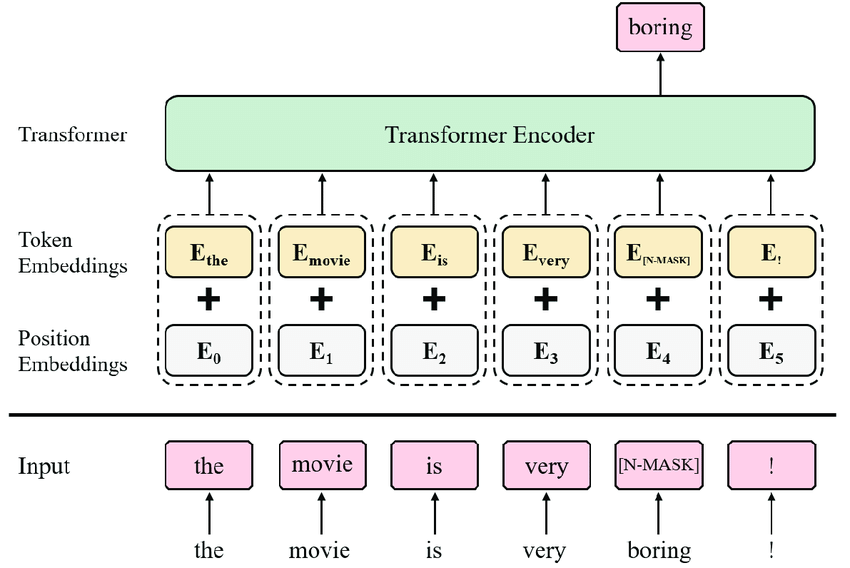
\includegraphics[width=0.9\textwidth]{images/llms/Model-structure-of-the-label-masked-language-model-N-MASK-is-a-mask-token-containing.png}
    \caption{An illustration of Masked Language Modeling (MLM) in a transformer architecture. The input sequence contains masked tokens that the model attempts to predict based on the context provided by the surrounding tokens. Token embeddings are combined with positional embeddings before being fed into the transformer encoder. The final output is a prediction of the masked token using the bidirectional context. \textit{Source:} \cite{park2019}}
    \label{fig:mlm_architecture}
\end{figure}

The introduction of MLM has significantly advanced the field of NLP. Models pre-trained with MLM have achieved state-of-the-art results on numerous benchmark datasets, demonstrating their effectiveness in capturing complex linguistic patterns. For example, BERT has set new performance standards on the General Language Understanding Evaluation (GLUE) benchmark \cite{wang2018glue}.

In addition, subsequent variations and extensions of the MLM approach, such as RoBERTa and XLNet, have further pushed the boundaries of what is possible with pre-trained language models \cite{liu2019roberta, yang2019xlnet}. These models have refined the MLM methodology, incorporating larger training corpora and more sophisticated training strategies to achieve even better results.

The choice between ALM and MLM during pre-training depends on the intended use of the LLM. In practice, combining these approaches can yield models that leverage the strengths of both, as seen in some recent advances in the field \cite{lewis2019bart}.

Understanding autoregressive and masked language modeling is fundamental to appreciating the design and capabilities of modern LLMs. These methods underpin the pre-training phase and set the stage for the remarkable performance of models in various NLP tasks.

Building on the foundational techniques of ALM and MLM, the next crucial aspect of pre-training large language models involves next-token and multi-token prediction, which play a pivotal role in enhancing the models’ predictive accuracy and contextual understanding.

\subsection{Next-Token Prediction and Multi-Token Prediction}

Next-token prediction is a fundamental task in training LLMs, where the model is trained to predict the next word in a sequence given the previous words. Formally, given a sequence of tokens \( \{x_1, x_2, \ldots, x_T\} \), the model learns to estimate the probability distribution \( P(x_t | x_1, x_2, \ldots, x_{t-1}) \). The learning objective is to minimize the cross-entropy loss:

\begin{equation}
    \mathcal{L}_1 = - \sum_{t} \log P_\theta (x_{t+1} | x_1, \ldots, x_t),
\end{equation}

where \( P_\theta \) is our LLM under training, aiming to maximize the probability of \( {x_{t+1}} \) as the next future token, given the history of past tokens \( {x_1, \ldots, x_t} \).

Recently, a novel methodology known as multi-token prediction has been proposed to improve the training efficiency and performance of LLMs. In this approach, the model predicts multiple future tokens simultaneously, rather than one token at a time. This method leverages a shared model trunk and multiple independent output heads to predict the next \( n \) tokens in parallel. This leads to the following factorization of the multi-token prediction cross-entropy
loss:

\begin{equation}
    \mathcal{L}_n = - \sum_{t} \sum_{i=1}^{n} \log P_\theta (x_{t+i} | z_{t:1}) \cdot P_\theta(z_{t:1} | x_{t:1}).
\end{equation}

In practice, as illustrated in Figure \ref{fig:multi-token-prediction}, the model architecture consists of a shared transformer backbone \( f_s \) that produces the hidden representation \( z_{t:1} \) from the observed context \( x_{t:1} \). Additionally, there are \( n \) independent output heads implemented as transformer layers \( f_{h_i} \), along with a shared unembedding matrix \( f_u \). Therefore, to predict \( n \) future tokens, the following it's computed:

\begin{equation}
    P_\theta(x_{t+i} | x_{t:1}) = \text{softmax}(f_u(f_{h_i}(f_s(x_{t:1})))),
\end{equation}

for \( i = 1, \ldots, n \), where specifically \( P_\theta(x_{t+1} | x_{t:1}) \) represents our next-token prediction head.

This multi-token prediction approach has demonstrated significant improvements in sampling efficiency and downstream performance, especially for larger model sizes and for tasks such as code generation. It has been shown that models trained with multi-token prediction can achieve higher accuracy on generative benchmarks such as HumanEval and MBPP, significantly outperforming models trained with traditional next-token prediction. In addition, multi-token prediction enhances the model's ability to perform algorithmic reasoning tasks and improves its out-of-domain generalization capabilities \cite{gloeckle2024better}.

\begin{figure}[h]
    \centering
    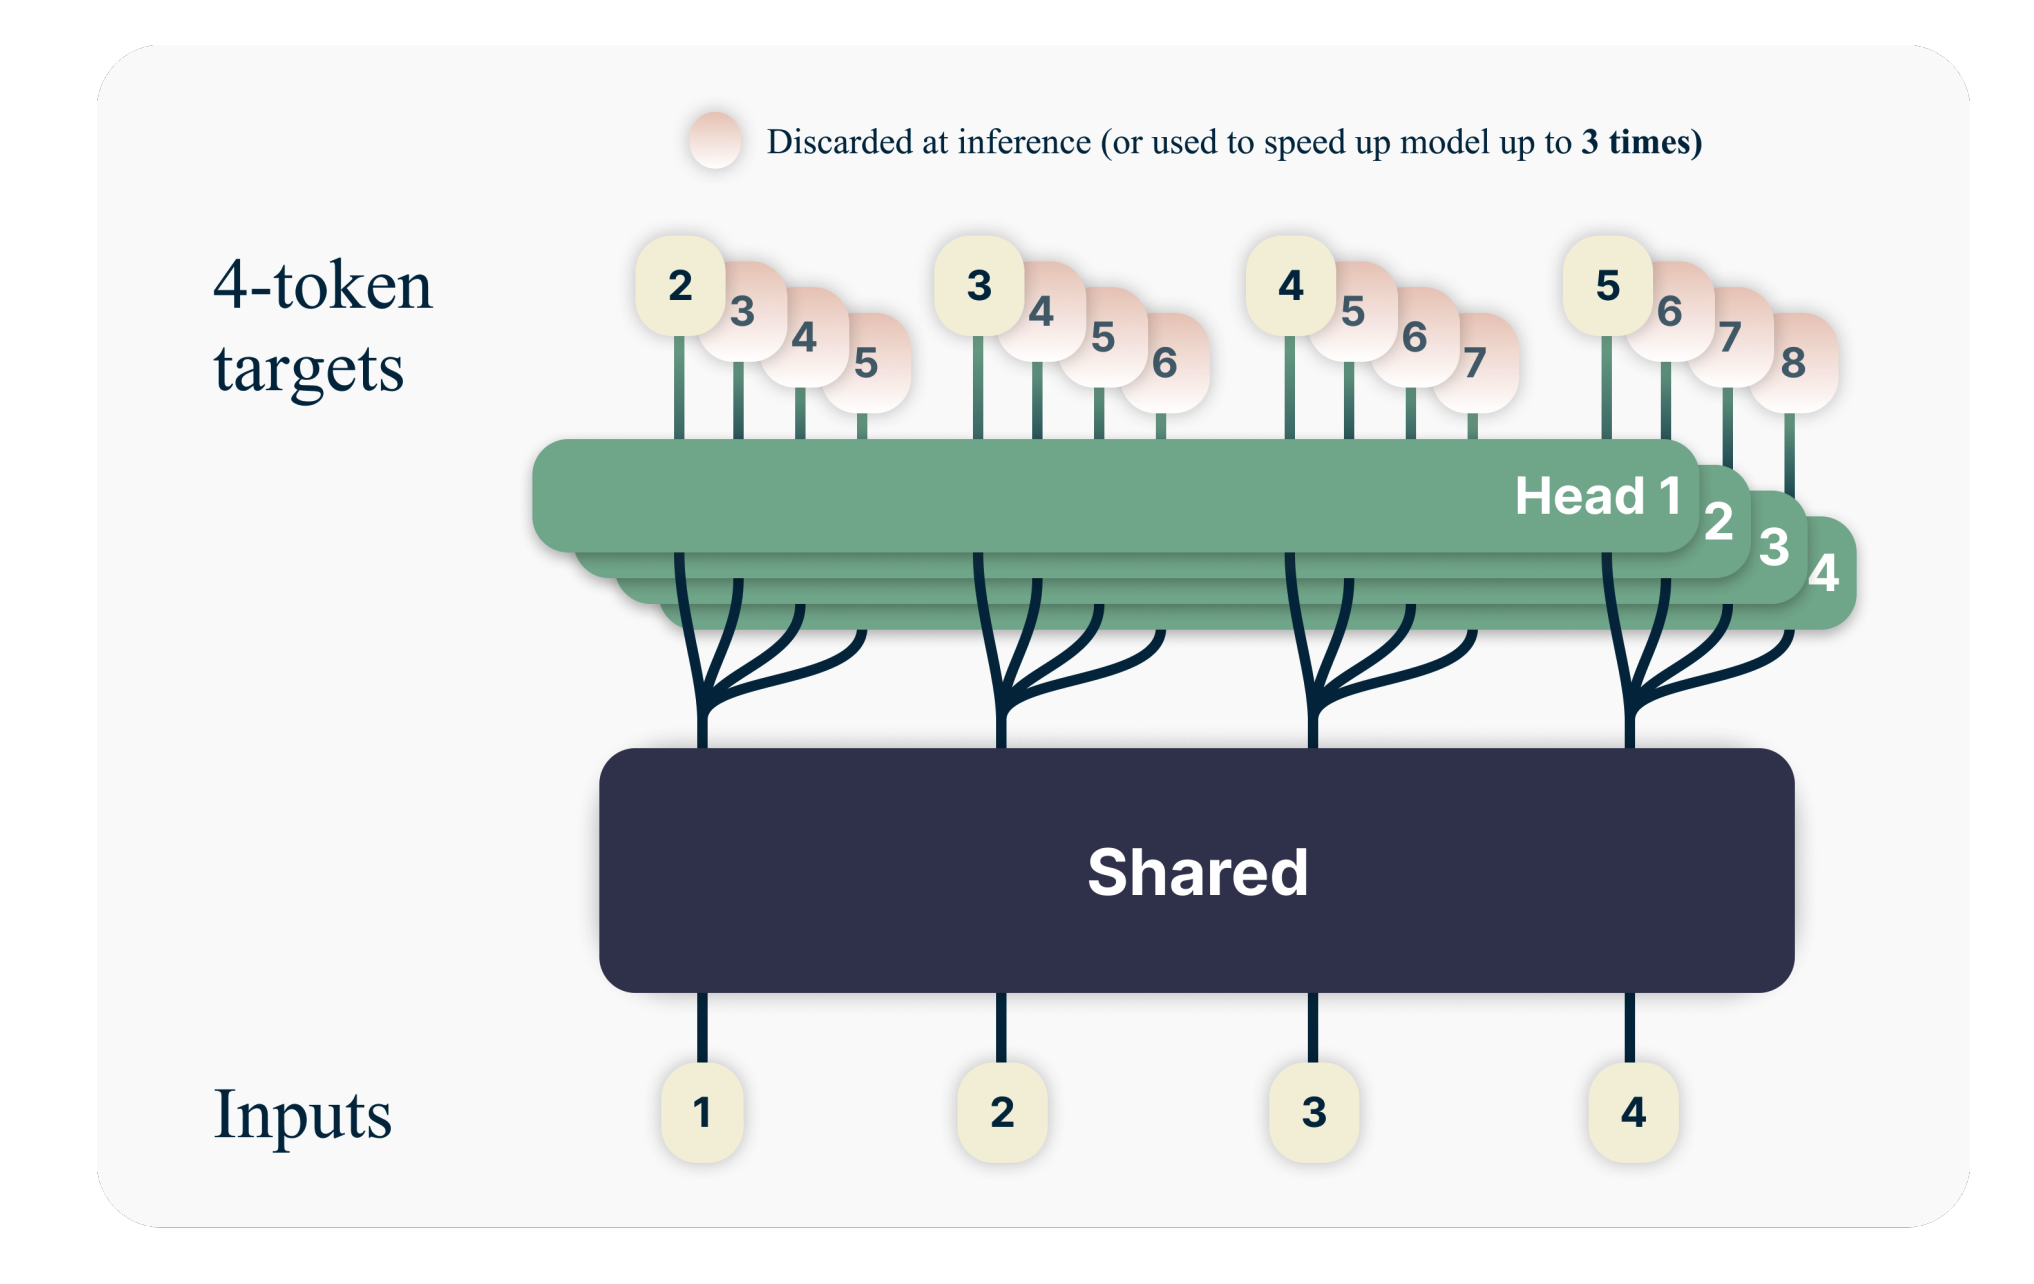
\includegraphics[width=0.9\textwidth]{images/llms/multi-token-pred-architecture.png}
    \caption{Overview of the Multi-Token Prediction Architecture. The model predicts four future tokens simultaneously using a common trunk and four independent output heads. This setup improves sampling efficiency and inference speed. The performance gains are particularly noticeable for larger models and for generative tasks. \textit{Source:} \cite{gloeckle2024better}}
    \label{fig:multi-token-prediction}
\end{figure}

Multi-token prediction offers a promising improvement over next-token prediction by allowing models to learn more efficiently and effectively. This methodology not only speeds up the training process, but also improves the overall performance of LLMs in various generative and reasoning tasks.

\section{Fine-tuning}

After the pre-training phase, the models are ready to be adapted to a variety of downstream tasks. This versatility and broad applicability underscore the foundational but incomplete nature of these models. For these and other reasons, these models are referred to as "foundation".

First, foundation models are critical to the advancement of AI by serving as the foundation on which more advanced models are built and refined. Their ability to address a wide variety of tasks in different domains, such as language, vision, robotics, reasoning, and human interaction, demonstrates their essential role in AI research and applications.

Second, the term "foundation" reflects the pivotal but evolving status of these models. Despite their impressive capabilities, they exhibit emergent properties that are not yet fully understood, and their large scale brings with it new, unanticipated capabilities. These models are based on deep learning and transfer principles, but their effectiveness across a wide range of tasks often leads to a degree of homogenization. While this uniformity offers significant advantages, it also means that any flaws or biases present in the underlying models are likely to be inherited by any downstream models adapted from them. \cite{bommasani2021opportunities}.

This adaptation phase is called fine-tuning and it constitutes a further training of the foundation model on narrower, domain-specific datasets. For instance, models can be fine-tuned on medical transcripts for healthcare applications or on legal briefs for legal assistant bots \cite{radford2019language}. Fine-tuning involves modifying the model’s weights to optimize its performance for the particular nuances and vocabulary of the task-specific data. This process entails adjusting the model's parameters (weights) according to the task-specific data, which often includes labeled examples for supervised tasks.

Fine-tuning can be improved with approaches such as Constitutional AI, which incorporates predefined rules into the model architecture, and reward training, in which humans evaluate the quality of multiple model outputs \cite{bai2022constitutional}. In addition, human feedback reinforced learning (RLHF), which uses a comparison-based system to optimize model responses, is employed. Although fine tuning is less computationally intensive, it requires significant human input to tune the model for specific tasks with predefined outputs. The optimized model is then used in a variety of applications, including chatbots \cite{ouyang2022training}.

\subsection{Methods of Fine-Tuning}

To tailor models for specific applications and optimize their performance, several fine-tuning techniques are employed, each with distinct advantages and suitable use cases. These methods allow for the adaptation of pre-trained models to meet the particular demands of new tasks.

\subsubsection{Full Model Fine-Tuning}

Full model fine-tuning represents the most straightforward approach, in which all parameters of the pre-trained model are updated during the fine-tuning process. This approach is particularly effective when the target task is very similar to the one on which the model was originally pre-tuned. The advantage of full model fine-tuning is its ability to adapt the model to the specific nuances of the new task, which can lead to improved performance \cite{howard2018universal}.

Nevertheless, the increasing size of LLMs over the years has rendered the fine-tuning process extremely computationally demanding and time-consuming. These challenges have significantly increased operational costs, and the financial burden of maintaining and deploying multiple instances of these fine-tuned models becomes especially pronounced when managing numerous downstream tasks.

In light of these challenges, alternative fine-tuning approaches, such as Parameter Efficient Fine-Tuning (PEFT) methods, have been developed with the objective of optimizing the process, thereby reducing the computational and financial burdens associated with full model fine-tuning. In particular, PEFT methods, in particular LoRA, will be discussed in detail in later sections.

\subsubsection{Layer-wise Fine-Tuning}
%%%
Layer-wise fine-tuning represents a more refined approach to model fine-tuning, whereby the model is fine-tuned in stages, starting with the top layers (closer to the output) and gradually incorporating lower layers (closer to the input). This method allows for more precise adaptation, which can be particularly advantageous when the target task necessitates only minor modifications to the pre-trained model. The application of layer-wise fine-tuning can serve to mitigate the issue of overfitting by limiting the extent of alterations made to the model's parameters. This approach is often utilized in scenarios where computational resources are constrained or when dealing with smaller datasets \cite{ro2021autolr}.

\subsubsection{Adapter Layers}

Adapter layers provide a flexible and efficient alternative to full model fine-tuning. In this technique, small neural network modules, referred to as "adapters," are inserted into the layers of the pre-trained model. During the fine-tuning process, only the parameters of the adapter layers are updated, while the original model parameters remain fixed. This approach markedly diminishes the number of parameters that require modification, consequently reducing computational costs and accelerating training times. Adapter layers have been demonstrated to perform at a comparable level to full model fine-tuning, particularly in low-resource settings. Furthermore, they have been shown to be highly effective for multi-task learning, where the same pre-trained model can be fine-tuned for different tasks by simply switching the adapters. \cite{houlsby2019parameter}.

\subsection{Parameter Efficient Fine-Tuning (PEFT)}

In order to address the considerable computational and financial costs associated with the vast scale of LLM systems, the parameter-efficient fine-tuning (PEFT) approach was developed as a viable solution to this challenge. This approach facilitates the efficient adaptation of large models to a range of downstream tasks, thereby reducing the burden of significant costs. PEFT entails the process of fine-tuning a pre-trained large model to a specific task or domain while minimizing the number of additional parameters introduced and the computational resources required \cite{han2024parameter}.

Among the various PEFT techniques, Low-Rank Adaptation (LoRA) is distinguished by its efficacy in reducing the computational demands associated with fine-tuning LLMs. For this reason, LoRA will be introduced in the following section.

\subsection{LoRA: Low-Rank Adaptation}

To address the increasing scale of models, Low-Rank Adaptation (LoRA) has been proposed. This method involves freezing the pre-trained model weights and incorporating trainable rank decomposition matrices into each layer of the Transformer architecture. This significantly reduces the number of trainable parameters required for downstream tasks. In comparison to fine-tuning GPT-3 175B using Adam, LoRA achieves a reduction in trainable parameters by a factor of 10,000 and decreases the GPU memory requirement by a factor of three.

Unlike traditional fine-tuning, which necessitates adjusting the entire model, LoRA focuses on modifying a smaller subset of parameters (lower-rank matrices), thereby reducing computational and memory overhead. This approach is predicated on the understanding that large models inherently possess a low-dimensional structure. By leveraging low-rank matrices, LoRA effectively adapts these models, allowing significant model changes to be represented with fewer parameters, thereby optimizing the adaptation process \cite{hu2021lora}.

\subsubsection{Decomposition in LoRA}

In traditional fine-tuning the weights of a pre-trained neural network are modified to adapt to a new task. This adjustment involves altering the original weight matrix \( W \) of the network. The changes made to \( W \) during fine-tuning are collectively represented by \( \Delta W \), such that the updated weights can be expressed as \( W + \Delta W \).

Rather than modifying \( W \) directly, the LoRA approach decomposes \( \Delta W \). This decomposition is crucial in reducing the computational overhead associated with fine-tuning large models.

The intrinsic rank hypothesis suggests that significant changes to the neural network can be captured using a lower-dimensional representation. Essentially, it posits that not all elements of \( \Delta W \) are equally important; instead, a smaller subset of these changes can effectively encapsulate the necessary adjustments.

Building on this hypothesis, LoRA represents \( \Delta W \) as the product of two smaller matrices, \( A \) and \( B \), with a lower rank. The updated weight matrix \( W' \) thus becomes:

\begin{equation}
    W' = W + BA
\end{equation}

In this equation, the variable \( W \) is held constant, indicating that it is not updated during the training process. The matrices \( B \) and \( A \) are of lower dimensionality, with their product \( BA \) representing a low-rank approximation of \( \Delta W \).

\begin{figure}[h]
    \centering
    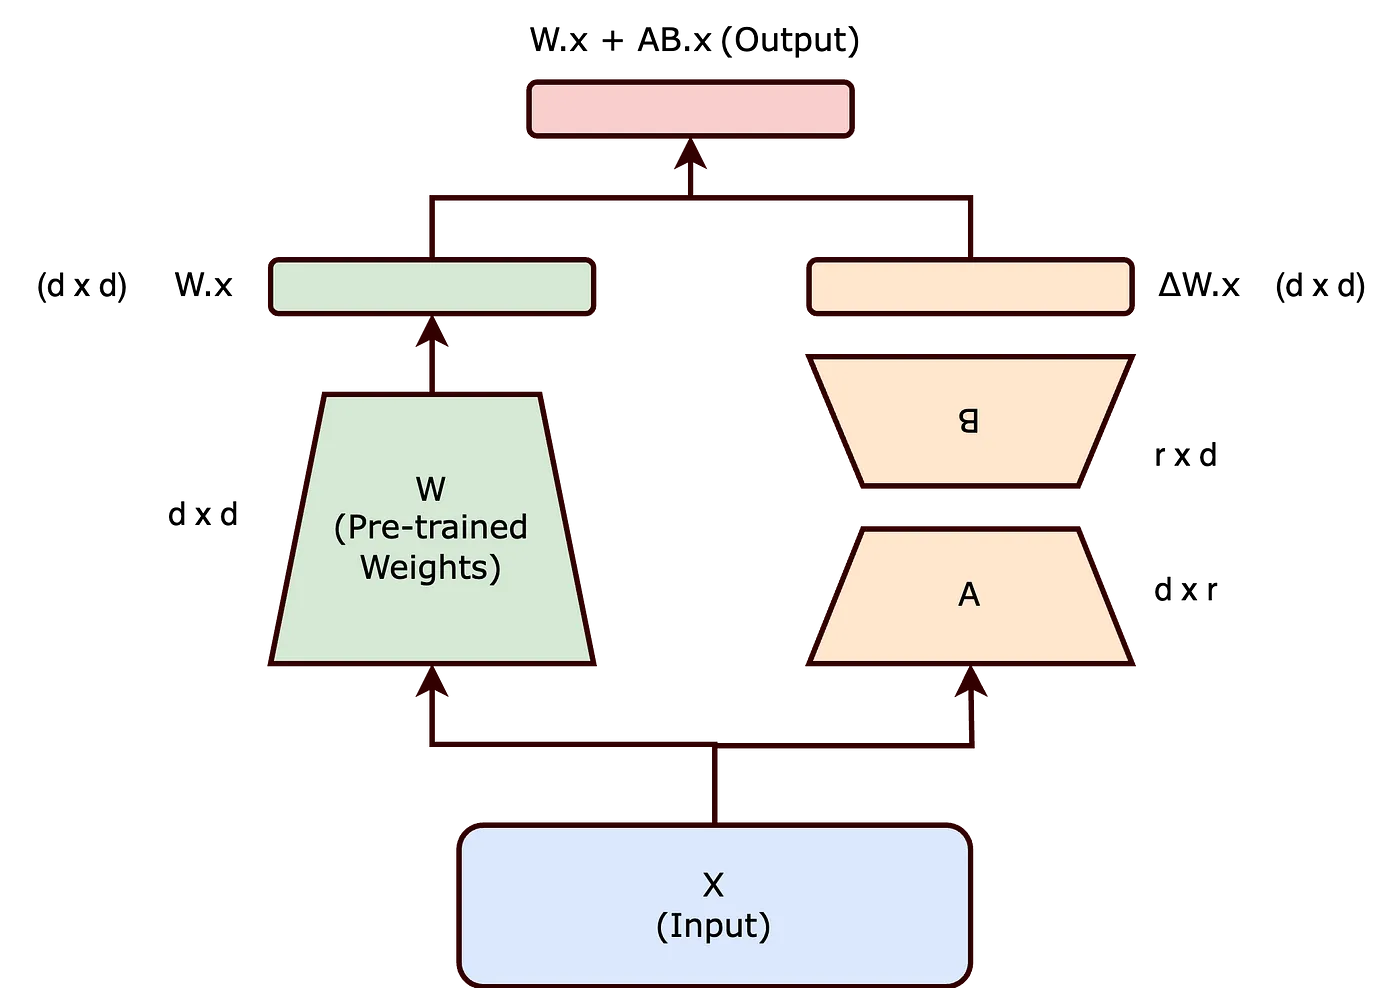
\includegraphics[width=0.9\textwidth]{images/llms/lora.png}
    \caption{Decomposition of \( \Delta W \) into two matrices \( A \) and \( B \), both of lower dimensionality than \( d \times d \). \textit{Source:} \cite{towardsdatascience2024lora}}
    \label{fig:lora_decomposition}
\end{figure}

As illustrated in Figure \ref{fig:lora_decomposition}, by choosing matrices \( A \) and \( B \) to have a lower rank \( r \), the number of trainable parameters is significantly reduced. For instance, if \( W \) is a \( d \times d \) matrix, traditionally, updating \( W \) would involve \( d^2 \) parameters. However, with \( B \) and \( A \) of sizes \( d \times r \) and \( r \times d \) respectively, the total number of parameters reduces to \( 2dr \), which is much smaller when \( r \ll d \) \cite{hu2021lora}. \newline

The reduction in the number of trainable parameters achieved through the LoRA method offers several significant advantages, particularly in the fine-tuning of large-scale neural networks. By lowering the number of parameters that need to be updated, LoRA reduces the system's memory footprint, which is crucial when managing extensive models. This reduction also leads to faster training and adaptation, as the computational demands are significantly diminished, allowing for more efficient training and fine-tuning of models for new tasks. Furthermore, the decreased parameter count makes it feasible to fine-tune large models on less powerful hardware, such as modest GPUs or CPUs, thereby broadening the accessibility of advanced AI capabilities. Finally, LoRA facilitates the scaling of AI models, enabling the expansion of their size and complexity without a corresponding increase in computational resources, thereby making the management of larger models more practical and cost-effective \cite{towardsdatascience2024lora}.

In the context of LoRA, the concept of rank plays a pivotal role in determining the efficiency and effectiveness of the adaptation process. Remarkably, the paper highlights that the rank of the matrices \( A \) and \( B \) can be astonishingly low, sometimes as low as one.

Despite the contributions of Hu et al. \cite{hu2021lora} primarily presents experiments in the field of NLP, the approach of low-rank adaptation is not limited to this domain and could be effectively employed in training various types of neural networks across different domains.

\section{Prompt-based Learning}

Prompt-based learning represents a significant shift in how LLMs are employed for natural language processing tasks. Instead of relying on extensive labeled datasets for training or fine-tuning, prompt-based learning uses textual prompts to guide the model in performing a specific task. This approach is particularly valuable in scenarios where the cost of annotating large datasets is prohibitive, such as in the development of AI chatbots for conversational AI \cite{madotto2021few}.

Prompt-based learning leverages the model's pre-trained knowledge by providing a prompt or instruction that directs the model's responses. The effectiveness of this technique has been demonstrated by works such as Radford et al. (2019) \cite{radford2019language} and Brown et al. (2020) \cite{brown2020language}, where prompt-based few-shot learning achieved results comparable to state-of-the-art models trained with full-shot datasets. This method relies on the model's ability to generalize from minimal examples (few-shot learning) or even without any examples (zero-shot learning), making it a versatile and cost-effective solution for various NLP tasks, including question answering and sentiment analysis.

\subsubsection{Prompt-Based Learning vs. Fine-Tuning}

The primary distinction between prompt-based learning and traditional fine-tuning lies in the training approach. While fine-tuning involves updating the model's weights based on a training set through a defined loss function, requiring substantial computational effort, prompt-based learning eliminates the need for this training phase altogether. Instead of modifying the model, prompt-based learning utilizes pre-defined prompts that instruct the model on how to perform a task without altering its weights. This makes prompt-based learning particularly advantageous in scenarios with limited computational resources or when rapid adaptation to new tasks is required, as it avoids the need for retraining \cite{madotto2021few}. 

\begin{figure}[h]
    \centering
    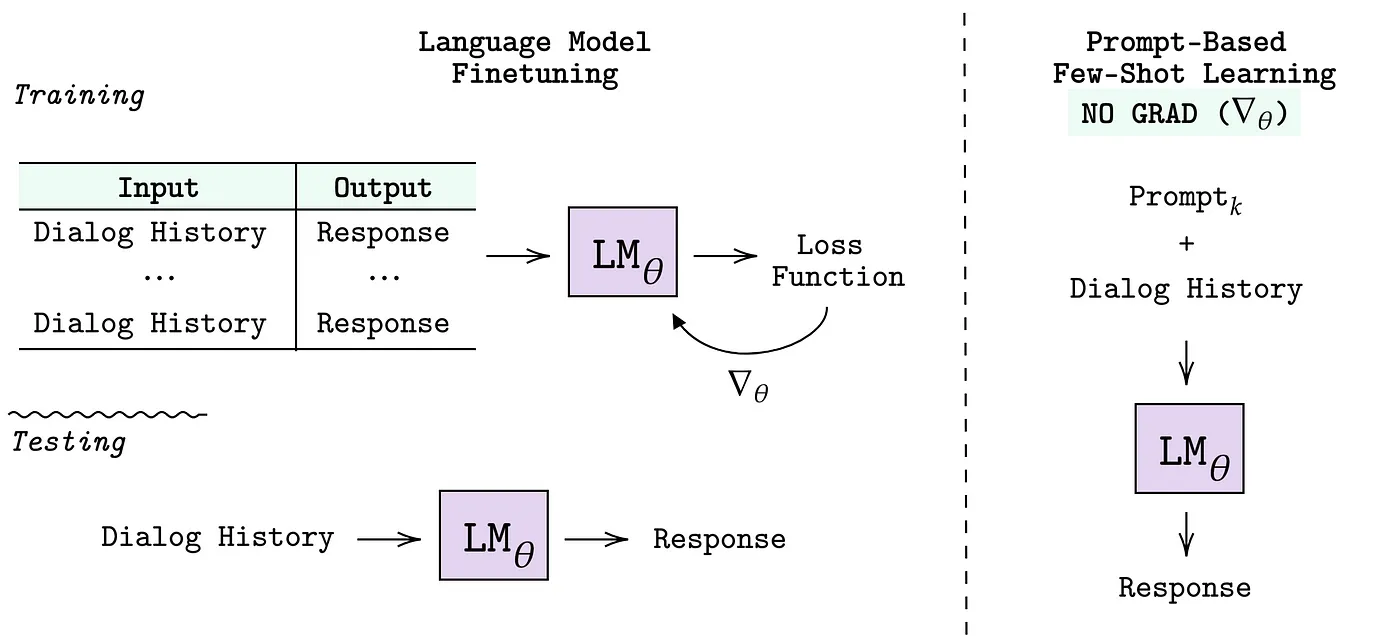
\includegraphics[width=0.9\textwidth]{images/llms/fine-tuning-vs-prompt-learning.png}
    \caption{Comparison of traditional fine-tuning (left) and prompt-based learning (right). In traditional fine-tuning, the model's weights are updated based on a training set, while in prompt-based learning, the model uses pre-defined prompts without altering its weights. \textit{Source:} \cite{madotto2021few}}
    \label{fig:fine_tuning_vs_prompt_learning}
\end{figure}

\subsection{Zero-Shot, One-Shot, and Few-Shot Learning}

Prompt-based learning is often implemented using zero-shot, one-shot, or few-shot prompts, each offering varying levels of example-based guidance to the model.

In Zero-Shot learning, the model is given a prompt to perform a task without any additional examples. The model relies solely on its pre-trained knowledge to generate a response, making zero-shot prompts highly efficient in scenarios where no task-specific data is available \cite{radford2019language}.

One-Shot learning involves providing the model with a single example in addition to the prompt. This example serves as a minimal guide, helping the model to generate responses that align more closely with the desired outcome.

Few-Shot learning extends this approach by supplying the model with a small number of examples (typically more than one but fewer than what would be used in full training). These examples, provided in the context of the prompt, help the model understand the task better, allowing it to produce responses that are more accurate and contextually appropriate \cite{brown2020language}.

\begin{figure}[h]
    \centering
    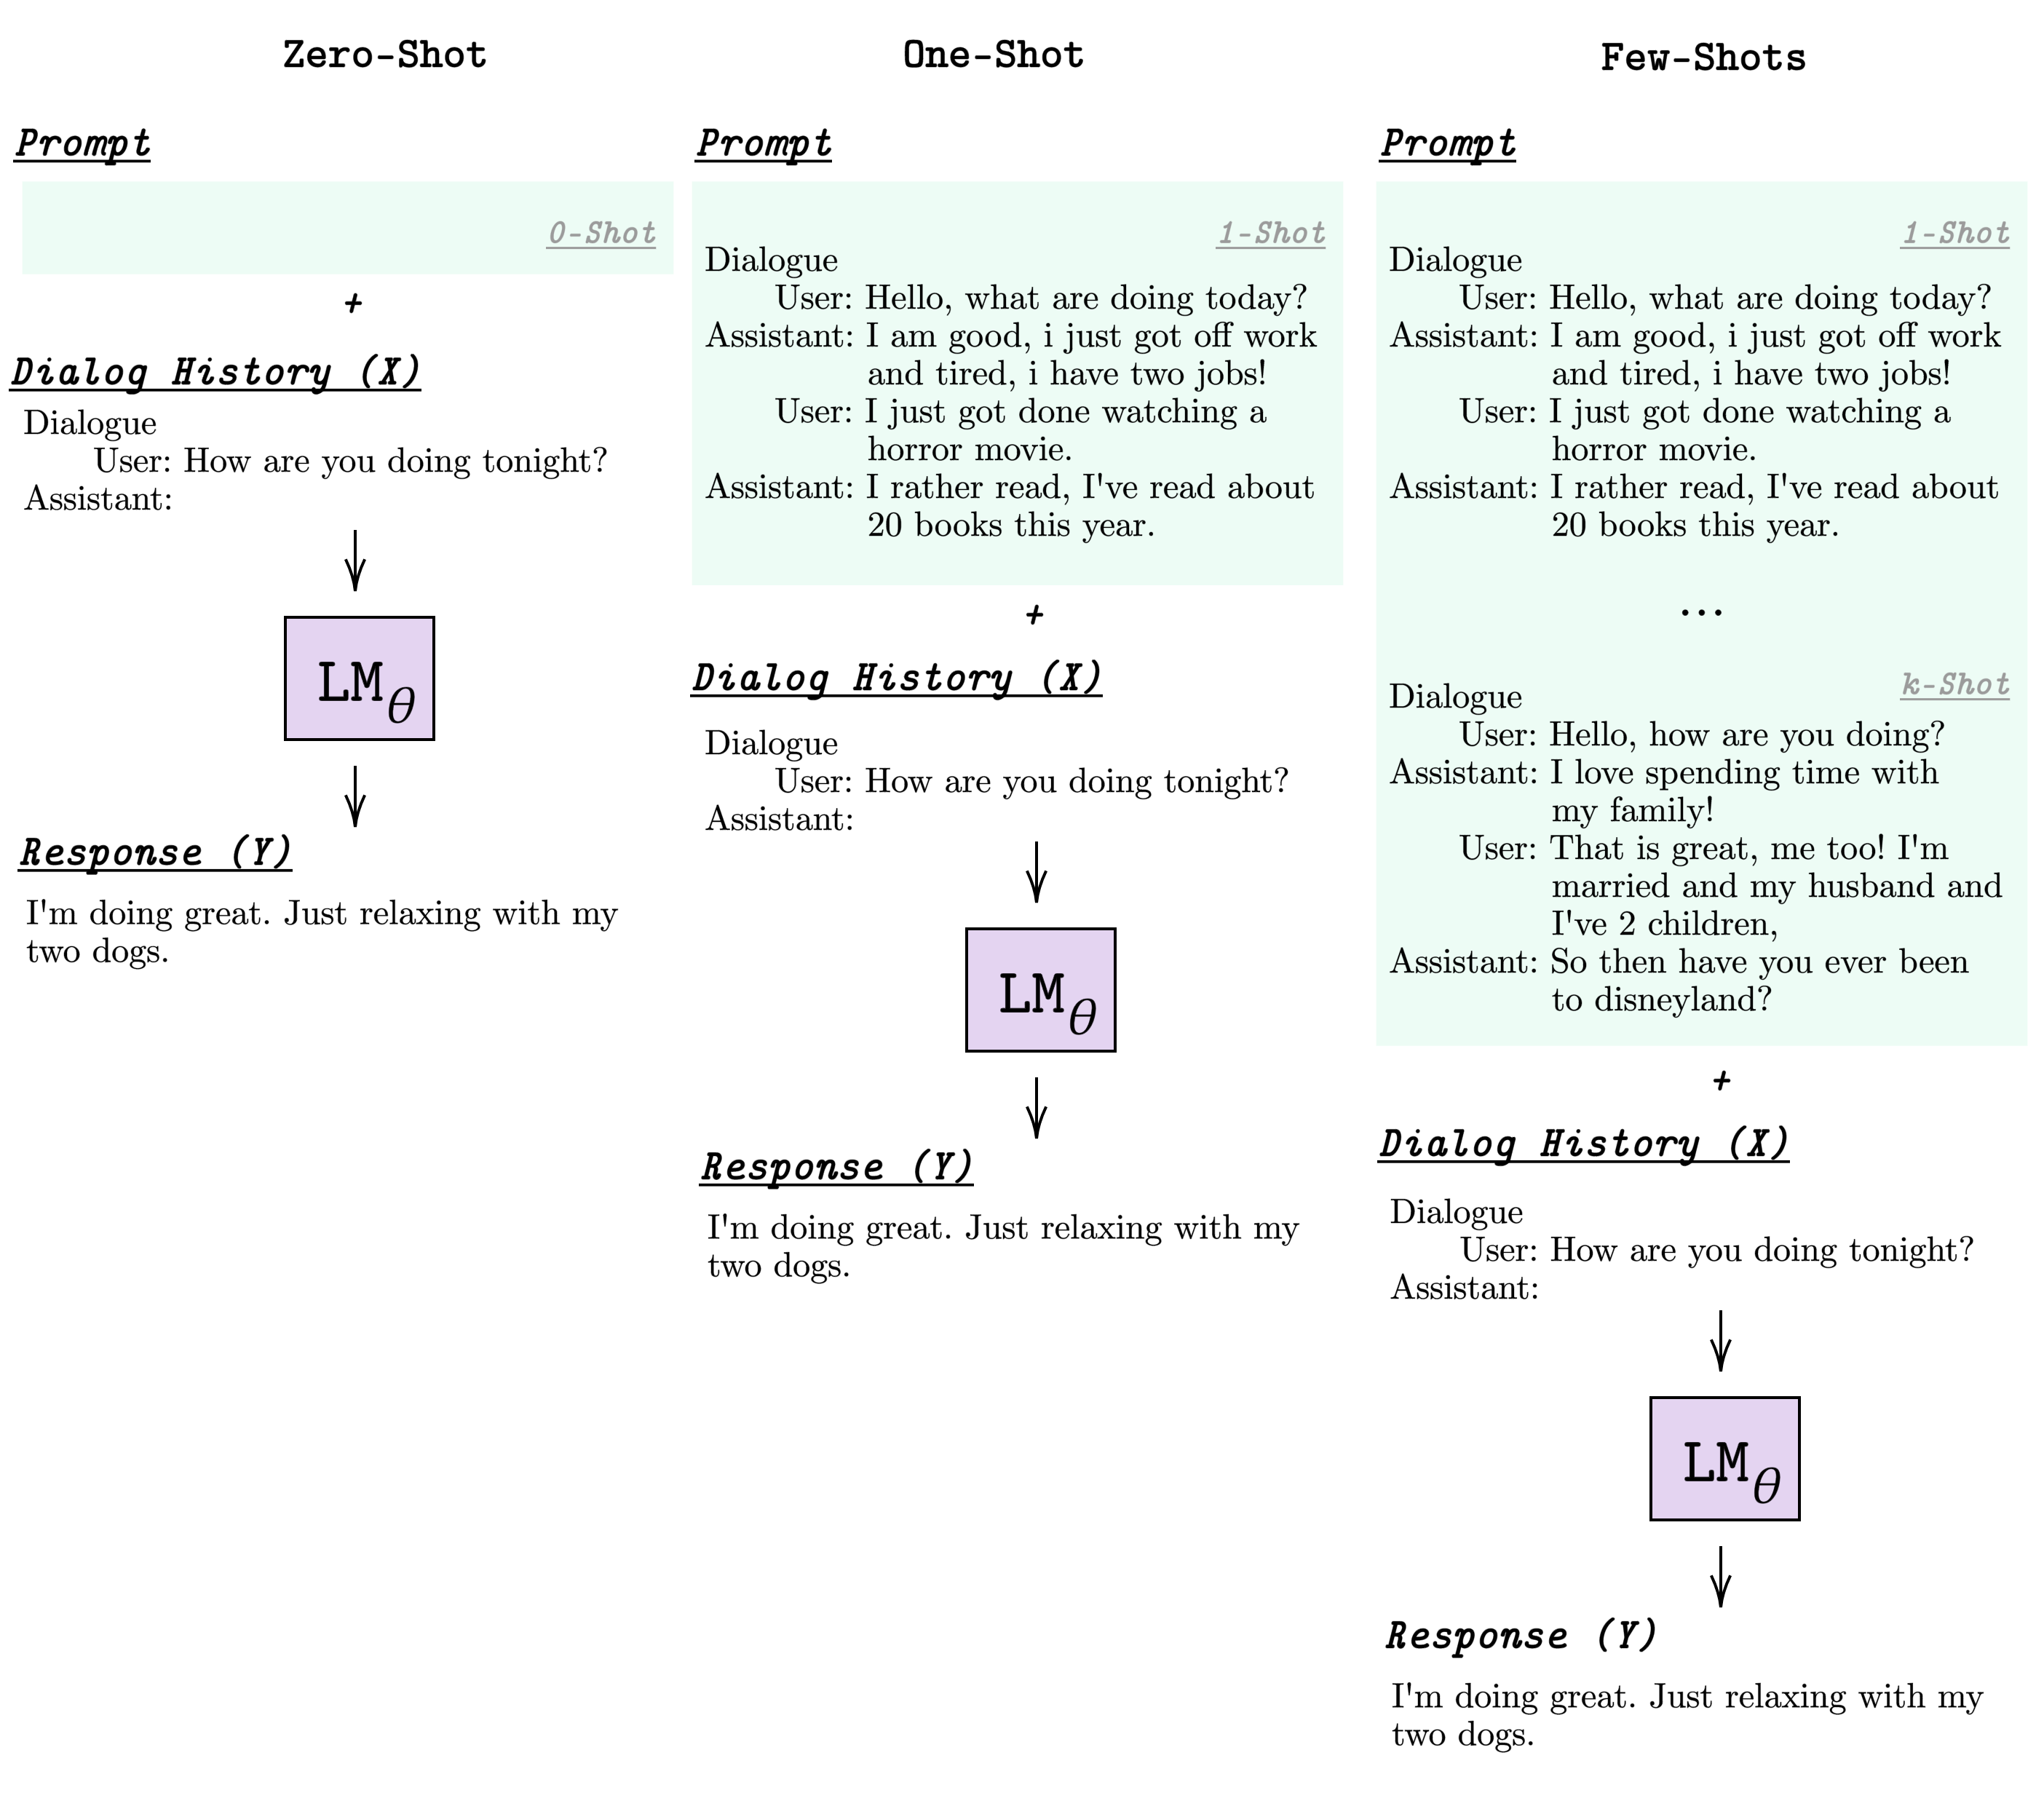
\includegraphics[width=0.9\textwidth]{images/llms/zero-one-few-shots.png}
    \caption{Illustration of Zero-Shot, One-Shot, and Few-Shot learning in dialogue systems. Zero-Shot learning involves no additional examples, One-Shot learning provides a single example, and Few-Shot learning includes a small number of examples to guide the model's response generation. \textit{Source:} \cite{madotto2021few}}
    \label{fig:zero_one_few_shot}
\end{figure}

As illustrated in Figure \ref{fig:zero_one_few_shot}, the effectiveness of prompt-based few-shot learning has been demonstrated across a wide range of tasks, including dialogue response generation, knowledge-grounded response generation, and dialogue state tracking. In many cases, it achieves performance comparable to, or even exceeding, that of fully fine-tuned models, without the need for extensive retraining. This makes prompt-based learning a powerful tool in the deployment of conversational AI systems, where flexibility and efficiency are paramount.

In conclusion, prompt-based learning offers a compelling alternative to traditional fine-tuning by allowing LLMs to perform specific tasks with minimal or no retraining. By utilizing zero-shot, one-shot, and few-shot prompts, this approach maximizes the utility of pre-trained models, making them more adaptable and cost-effective in a wide variety of applications.

\subsection{Chain of Thought Prompting}

In recent years, more advanced techniques have emerged, with one particularly promising approach being Chain-of-Thought (CoT) prompting.

Chain-of-Thought reasoning represents a methodology designed to enhance the reasoning capabilities of large language models by directing them to construct a sequence of intermediate steps that collectively culminate in a final answer. This approach emulates the natural human thought process when addressing complex tasks, such as multi-step mathematical problems, where the problem is decomposed into smaller, more tractable components before reaching a solution.

As illustrated in Figure \ref{fig:cot_reasoning}, Chain of Thought reasoning allows language models to handle complex reasoning tasks more effectively by decomposing the problem into intermediate stages. For example, when solving a math word problem, a model might generate a sequence of logical steps that resemble the way a human might solve the problem step-by-step: “After Jane gives 2 flowers to her mom, she has 10 left… then after giving 3 to her dad, she will have 7… so the answer is 7.” This sequential reasoning helps the model arrive at the correct answer by focusing on each part of the problem individually.

\begin{figure}[h]
    \centering
    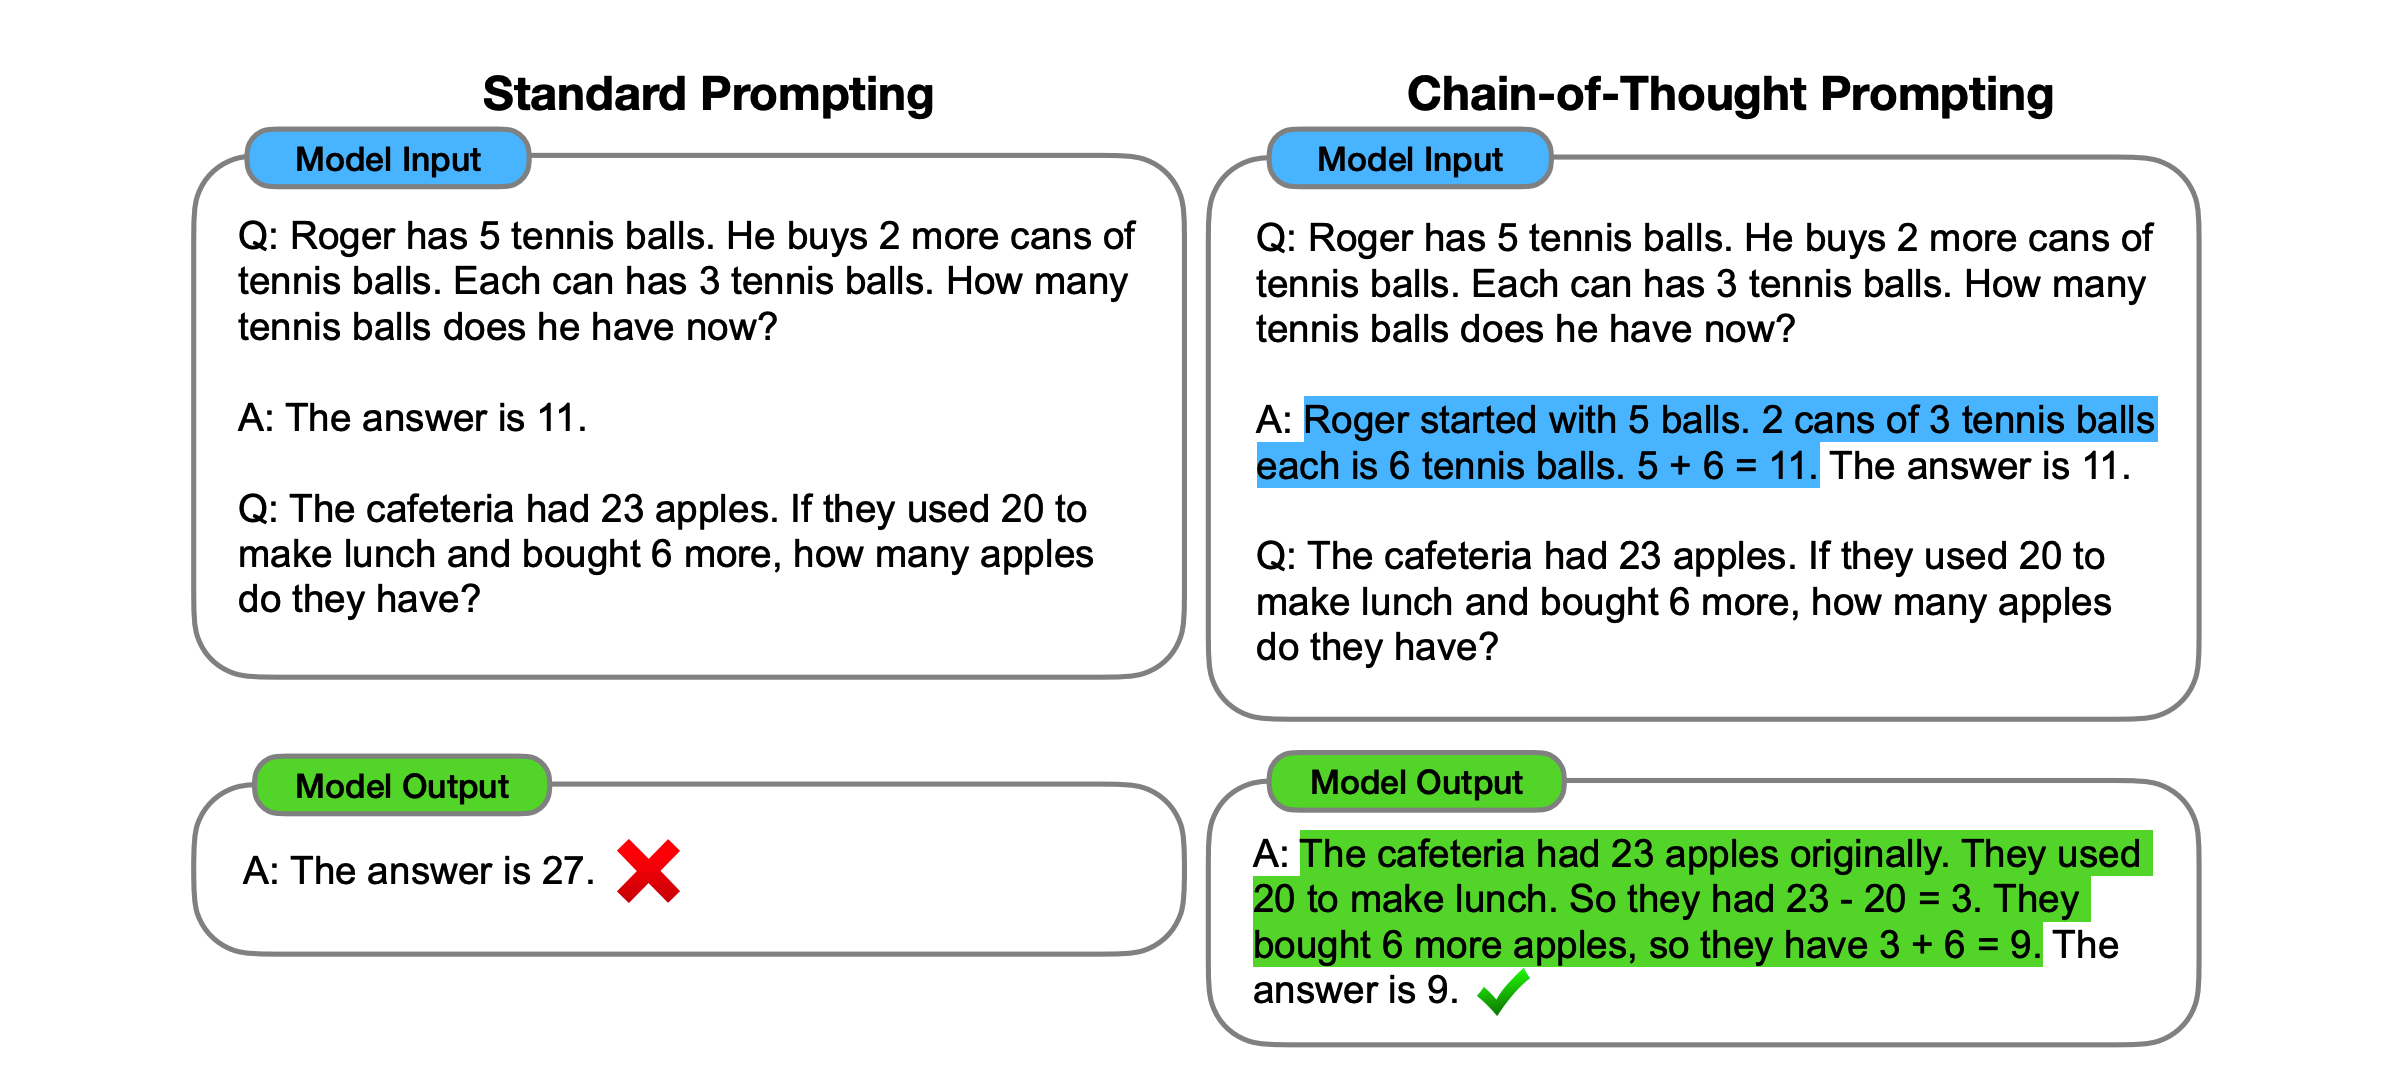
\includegraphics[width=0.9\textwidth]{images/llms/cot-resoning.png}
    \caption{Comparison of standard prompting and Chain-of-Thought (CoT) prompting. The CoT approach allows the model to break down problems into intermediate steps, leading to more accurate and interpretable outcomes.}
    \label{fig:cot_reasoning}
\end{figure}

One of the significant advantages of Chain of Thought reasoning is its interpretability. By breaking down the reasoning process into a series of intermediate steps, CoT provides insights into how the model arrived at a particular answer. This not only helps in understanding the model’s decision-making process but also offers opportunities to identify and correct errors in the reasoning path.

Moreover, Chain of Thought reasoning is versatile and can be applied to a variety of tasks that require complex reasoning, such as solving math word problems, engaging in commonsense reasoning, and performing symbolic manipulation. Essentially, it can be applied to any task where humans typically solve problems through language-based reasoning.

Another notable benefit of Chain of Thought prompting is that it can be effectively elicited in large language models by incorporating examples of such reasoning into the few-shot prompting process. This means that without any additional fine-tuning, sufficiently large pre-trained models can generate these reasoning chains simply by being provided with relevant examples during the prompting phase \cite{wei2022chain}.

In summary, Chain of Thought reasoning represents a powerful tool for enhancing the reasoning capabilities of language models. By breaking down complex problems into intermediate steps, it not only improves the accuracy of the model’s outputs but also provides a transparent and interpretable reasoning process that can be applied across a wide range of tasks.

\subsection{Instruction Prompt Tuning}

% ----------------------- Read from here  -----------------------

An innovative technique, instruction prompt tuning, introduced by Lester et al. \cite{lester2021power}, provides a cost-effective solution to update the model's parameters, thereby improving performance in numerous downstream tasks. Instruction prompt tuning offers significant advantages over few-shot prompting, particularly for clinical applications, because it allows LLMs to be more effectively aligned with the specific requirements of the medical domain, as demonstrated by Singhal et al. \cite{singhal2022large}

Prompt tuning is designed to improve the performance of frozen language models on specific downstream tasks by learning so-called "soft prompts". Unlike traditional discrete text prompts, which are manually selected or searched for, soft prompts are learned through backpropagation, allowing them to be fine-tuned based on labeled examples.

At a high level, prompt tuning shifts the focus from tuning the entire model to tuning only the parameters of the prompts. This approach involves conditioning a frozen language model on these soft prompts to guide its output generation, thereby enhancing the model's ability to perform specific tasks. This is particularly important because it allows the use of large pre-trained models without the need to modify their core weights, making the approach both resource efficient and scalable.

The concept of prompt tuning builds on the idea of conditioning models with additional information. Typically, in models such as GPT-3, prompts are added as additional tokens that the model uses to generate the desired output. However, these tokens are part of the model's fixed embedding space, which means that they cannot be directly optimized by training. Prompt tuning overcomes this limitation by introducing dedicated parameters for the prompts themselves, which can be updated during training.

As a result, prompt tuning becomes increasingly competitive as the size of the language model grows. Remarkably, it can match the performance of full model tuning - where all model weights are adjusted - even when the model size reaches billions of parameters. This makes prompt tuning a powerful tool, especially for large models where fine-tuning all parameters is computationally expensive and impractical.

In addition, prompt tuning has demonstrated advantages in robustness to domain transfer and offers the flexibility of "prompt ensembling," where multiple prompts can be combined to improve performance. This approach also simplifies the process of adapting a single frozen model to multiple downstream tasks, reducing the need to deploy and manage multiple fine-tuned models. \cite{lester2021power}

In summary, prompt tuning is a highly effective method for improving the performance of large language models on specific tasks by learning and tuning soft prompts. This approach not only simplifies the tuning process, but also maintains the efficiency and scalability of using frozen, pre-trained models across different applications. 

\section{Limitations of Large Language Models in Practical Applications}

After examining LLMs, their architecture, and the impact of model size on AI performance, as well as exploring various training and fine-tuning methods, including prompt-based learning techniques, it is essential to address the limitations of these models in practical applications.

One of the most significant limitations of LLMs is their lack of transparency in predictions. The models operate as black boxes, making it difficult to interpret the reasoning behind their outputs. This opacity is problematic, especially when LLMs are used in decision-making processes that require accountability and traceability \cite{rudin2019stop}.

Another critical issue is the tendency of LLMs to produce “hallucinations”—statements that are plausible but factually incorrect. These hallucinations arise because LLMs generate text based on patterns learned from vast amounts of data, without a deep understanding of the world or the ability to fact-check their outputs \cite{maynez2020faithfulness}. This risk is exacerbated by the fluency and coherence of the generated text, which can mislead users into accepting false information as true.

Bias is another well-documented limitation of LLMs. These models can inadvertently perpetuate and amplify biases present in the training data, leading to outputs that reinforce stereotypes or discriminate against certain groups \cite{bender2021dangers}. This bias is particularly concerning in applications like hiring, lending, or law enforcement, where fairness and impartiality are paramount.

Additionally, LLMs face issues of staleness and revisions. Since these models are trained on static datasets, they cannot incorporate new information that emerges after their training, leading to outdated or incorrect responses \cite{dhingra2022time}. Furthermore, the accuracy of information retrieval is another challenge, as LLMs often struggle to retrieve specific, relevant information from their vast learned knowledge, leading to irrelevant or imprecise responses.

The limitations mentioned above significantly undermine the reliability and value of LLMs in practical applications. When these models generate inaccurate or misleading outputs, the consequences can be severe, especially in critical fields where precision and factual correctness are essential.

To address these limitations, one promising approach is Retrieval-Augmented Generation (RAG). RAG enhances the capabilities of LLMs by integrating an external retrieval mechanism that allows the model to access and utilize up-to-date and contextually relevant information during the generation process \cite{lewis2020retrieval}. This method mitigates issues related to staleness, hallucinations, and factual inaccuracies by grounding the model’s outputs in verifiable external sources, thereby improving the accuracy and reliability of its responses. As a result, RAG offers a viable solution to many of the challenges faced by LLMs in practical applications, making them more effective and trustworthy in real-world scenarios.

\section{Retrieval-Augmented Generation (RAG)}

To address the discussed challenges, Meta AI researchers introduced a method called Retrieval-Augmented Generation (RAG) \cite{lewis2020retrieval}. RAG is a powerful technique that enhances LLMs by integrating them with external knowledge sources, operating by retrieving relevant document chunks from an external knowledge base through semantic similarity calculations. By referencing external knowledge, RAG effectively reduces the occurrence of hallucinations and improves the factual accuracy of the generated content. This integration has led to widespread adoption of RAG, establishing it as a key technology in advancing AI applications like chatbots and enhancing the suitability of LLMs for real-world scenarios.

The development of RAG technology has progressed rapidly, evolving through distinct stages. Initially, the inception of RAG coincided with the rise of the Transformer architecture, focusing on enhancing language models by incorporating additional knowledge through Pre-Training Models (PTM). This early stage was characterized by foundational work aimed at refining pre-training techniques \cite{arora2023gar, lewis2020retrieval, borgeaud2022improving}. 

The subsequent arrival of models like ChatGPT marked a pivotal moment, showcasing powerful in-context learning (ICL) capabilities. RAG research shifted towards providing better information for LLMs to tackle more complex and knowledge-intensive tasks during the inference stage. As research progressed, RAG's enhancement was no longer limited to the inference stage but began to incorporate more with LLM fine-tuning techniques.

A typical application of RAG is illustrated in Figure \ref{fig:rag_example}. In this example, a user poses a question to ChatGPT about a recent news event. Given that ChatGPT relies on pre-training data, it initially lacks the ability to provide updates on recent developments. RAG bridges this information gap by sourcing and incorporating knowledge from external databases. In this case, relevant news articles related to the user's query are retrieved and combined with the original question to form a comprehensive prompt, empowering the LLM to generate a well-informed answer.

\begin{figure}[h]
    \centering
    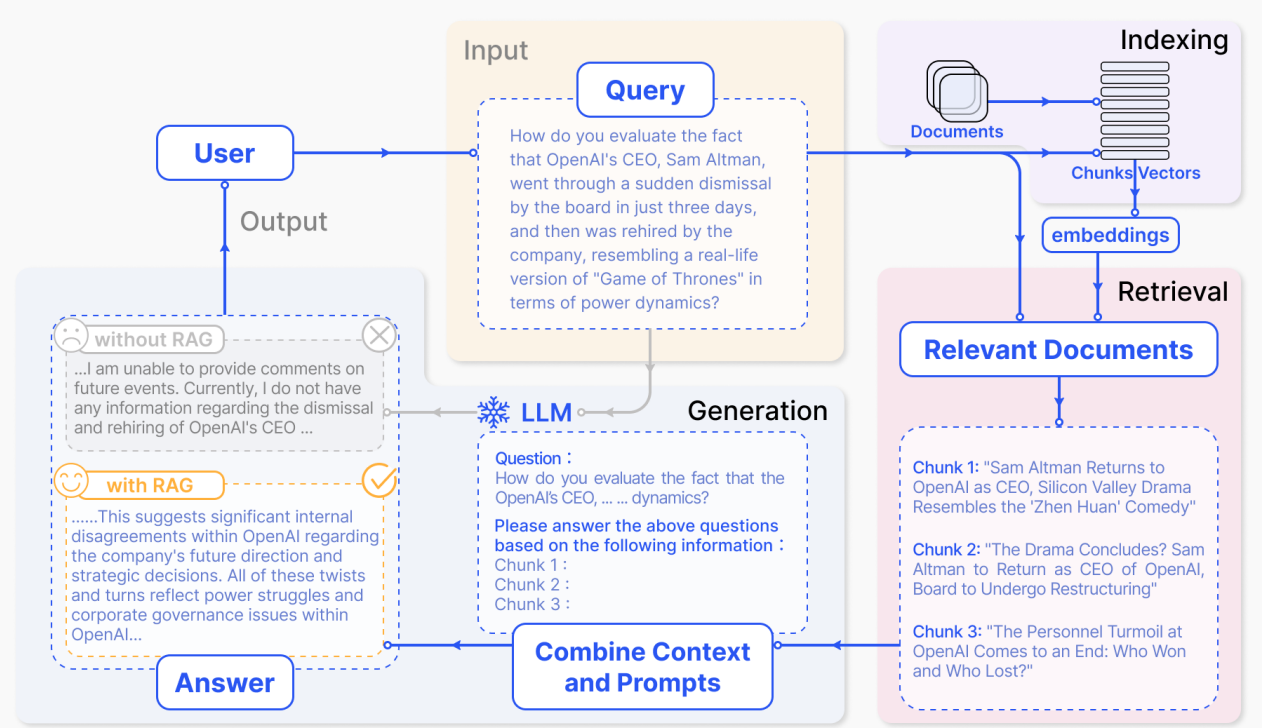
\includegraphics[width=0.9\textwidth]{images/llms/rag-strategies.png}
    \caption{A representative instance of the RAG process applied to question answering. It consists of three main steps: 1) Indexing, where documents are split into chunks, encoded into vectors, and stored in a vector database. 2) Retrieval, where the top-K chunks most relevant to the question are retrieved based on semantic similarity. 3) Generation, where the original question and the retrieved chunks are input together into the LLM to generate the final answer. \textit{Source:} \cite{gao2023retrieval}}
    \label{fig:rag_example}
\end{figure}

As RAG continues to evolve, we can categorize its development into three stages: Naive RAG, Advanced RAG, and Modular RAG. Although RAG methods are cost-effective and surpass the performance of native LLMs, they also exhibit certain limitations. The development of Advanced RAG and Modular RAG represents a response to these specific shortcomings in the Naive RAG stage \cite{gao2023retrieval}.

\subsubsection{Naive RAG}

The Naive Retrieval-Augmented Generation (RAG) approach represents the foundational methodology in RAG systems and gained prominence following the widespread adoption of models like ChatGPT. Naive RAG follows a straightforward "Retrieve-Read" framework \cite{ma2023query}, which typically involves three critical phases: indexing, retrieval, and generation.

\textbf{Indexing} is the initial phase where raw data from various formats, such as PDFs, HTML, Word documents, and Markdown files, are cleaned and converted into a uniform plain text format. Given the context limitations of language models, the text is then segmented into smaller, manageable chunks. These chunks are encoded into vector representations using an embedding model and stored in a vector database. This process is crucial as it lays the groundwork for efficient similarity searches during the retrieval phase.

\textbf{Retrieval} begins when a user query is submitted. The system utilizes the same encoding model used during indexing to transform the query into a vector representation. The system then computes similarity scores between the query vector and the vectors of chunks within the indexed corpus. The top K chunks with the highest similarity scores are retrieved and used as the expanded context for the prompt.

\textbf{Generation} involves synthesizing the user’s query with the retrieved documents to create a coherent prompt, which the large language model uses to generate a response. Depending on task-specific criteria, the model might draw on its parametric knowledge or restrict its response to the retrieved documents. However, Naive RAG faces several significant challenges, including issues with retrieval precision and recall, and the generation of content that may suffer from hallucinations, irrelevance, or bias \cite{gao2023retrieval}.

\subsubsection{Advanced RAG}

Advanced RAG builds on the foundational Naive RAG framework by introducing specific improvements designed to address the limitations observed in the earlier model. This approach enhances the quality of retrieval by implementing both pre-retrieval and post-retrieval strategies, focusing on refining the indexing process and optimizing how queries are handled.

In the pre-retrieval phase, the emphasis is on optimizing the structure of the index and refining the original user query to improve retrieval quality. Strategies such as the sliding window approach, fine-grained text segmentation, and the incorporation of metadata are employed to enhance the granularity and relevance of the indexed content \cite{ilin2023advancedrag}. Additionally, query optimization techniques such as query rewriting, transformation, and expansion are used to ensure the query is well-suited for effective retrieval.

The post-retrieval phase focuses on integrating the retrieved context more effectively with the user’s query. Key methods include re-ranking the retrieved chunks to prioritize the most relevant information and compressing the context to avoid information overload when feeding it into the language model. These strategies help address the generation challenges encountered in Naive RAG by ensuring that the final output is more focused, relevant, and coherent.

Advanced RAG’s systematic enhancements to both the indexing and retrieval processes significantly improve the overall performance of RAG systems, making them more robust and capable of handling complex queries with greater accuracy \cite{gao2023retrieval}.

\subsubsection{Modular RAG}

Modular RAG represents the next evolution in the RAG paradigm, offering a more flexible and adaptable architecture that can be customized to meet the needs of a wide range of tasks and scenarios. This approach builds upon the foundational principles of Naive and Advanced RAG but introduces modular components that can be independently optimized and reconfigured.

\textbf{New Modules} are a key feature of Modular RAG. This architecture incorporates specialized components designed to enhance retrieval and processing capabilities. For instance, the \textbf{Search module} allows for direct searches across diverse data sources, such as search engines, databases, and knowledge graphs, using LLM-generated code and query languages \cite{wang2023knowledgpt}. The \textbf{RAGFusion module} addresses the limitations of traditional search by employing a multi-query strategy that expands user queries into diverse perspectives, utilizing parallel vector searches and intelligent re-ranking to uncover both explicit and transformative knowledge \cite{ragfusion2023}. Additionally, the \textbf{Memory module} leverages the language model’s memory to guide retrieval, creating an unbounded memory pool that iteratively enhances the alignment between text and data distribution \cite{cheng2024lift}.

The \textbf{Routing module} in Modular RAG optimizes query pathways by navigating through various information sources, selecting the most appropriate route for each query. This might involve summarization, specific database searches, or merging different information streams to provide a comprehensive response \cite{li2023classification}. The \textbf{Predict module} reduces redundancy and noise by generating context directly within the LLM, ensuring that the outputs are relevant and accurate \cite{yu2022generate}. Finally, the \textbf{Task Adapter module} tailors the RAG system to various downstream tasks, automating prompt retrieval for zero-shot inputs and creating task-specific retrievers through few-shot query generation \cite{cheng2023uprise}.

\textbf{New Patterns} in Modular RAG provide remarkable adaptability by allowing for module substitution or reconfiguration to address specific challenges. Unlike the fixed structures of Naive and Advanced RAG, Modular RAG offers the flexibility to integrate new modules or adjust the interaction flow among existing ones, enhancing its applicability across different tasks. Innovations such as the \textbf{Rewrite-Retrieve-Read} model and the \textbf{Demonstrate-Search-Predict} (DSP) framework illustrate how Modular RAG can leverage LLMs capabilities to refine retrieval queries and improve task performance \cite{khattab2022demonstrate}.

Modular RAG’s dynamic architecture not only simplifies the retrieval process but also significantly enhances the quality and relevance of the information retrieved. Its flexibility allows for the integration of other technologies, such as fine-tuning or reinforcement learning, further expanding its effectiveness and adaptability in diverse application scenarios.

\begin{figure}[h]
    \centering
    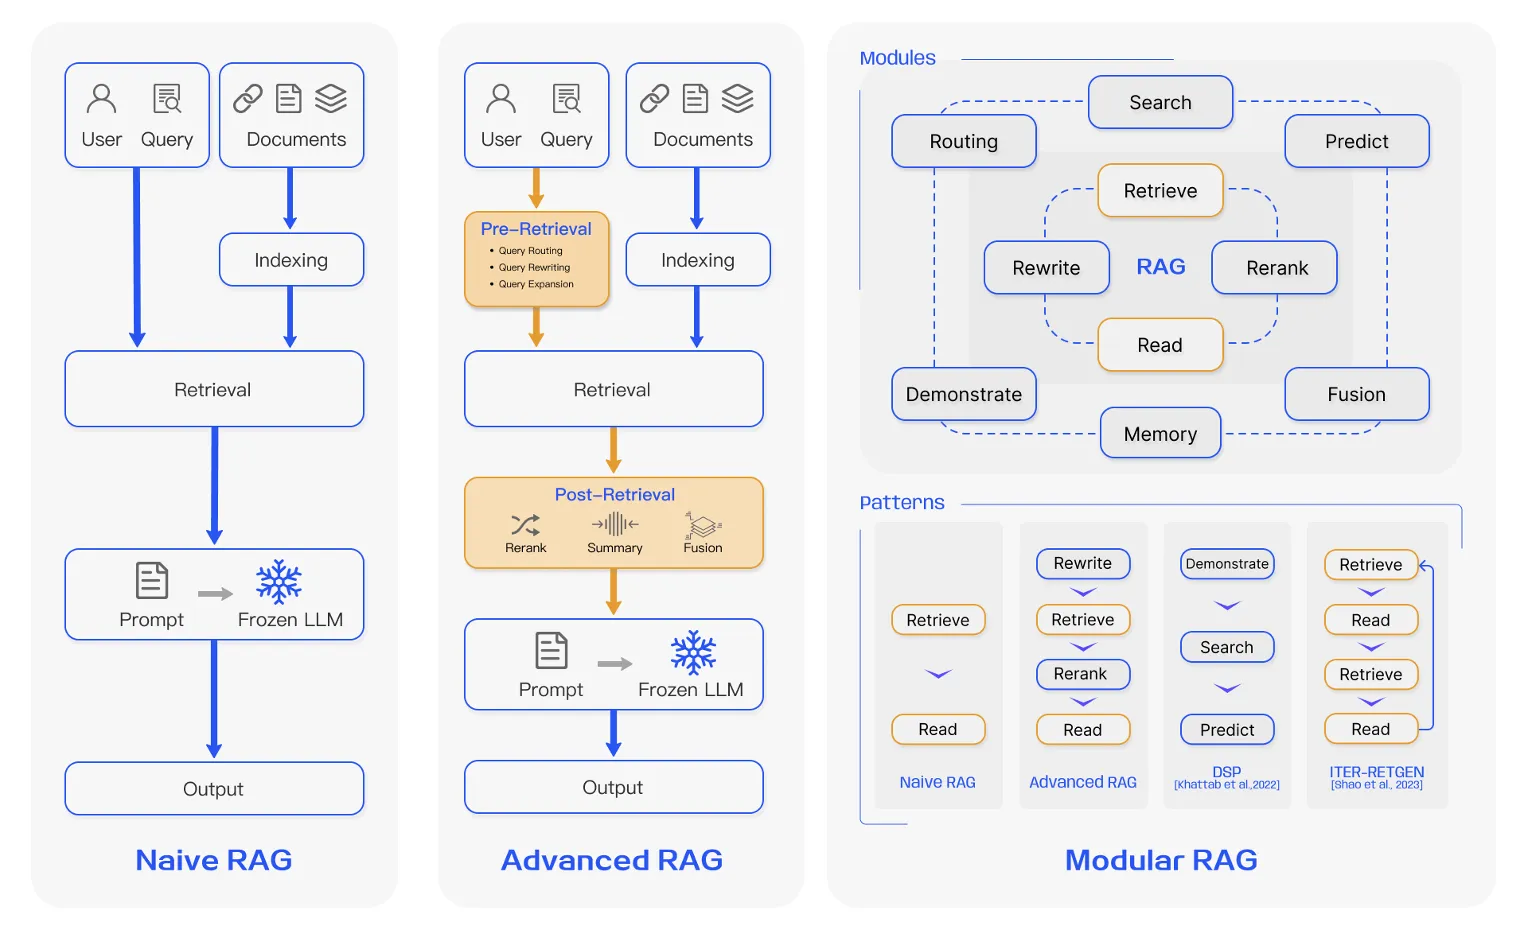
\includegraphics[width=0.9\textwidth]{images/llms/naive-adv-modular-rag.png}
    \caption{Comparison between the three paradigms of RAG. Naive RAG (left) consists of three parts: indexing, retrieval, and generation. Advanced RAG (middle) introduces multiple optimization strategies around pre-retrieval and post-retrieval, while Modular RAG (right) develops from the previous paradigms, showcasing greater flexibility with the introduction of multiple specific functional modules. \textit{Source:} \cite{gao2023retrieval}}
    \label{fig:rag_paradigms}
\end{figure}

In summary, Modular RAG represents a significant advancement in the development of RAG systems, offering a highly adaptable and modular architecture that addresses the limitations of earlier models while providing the flexibility needed to tackle a wide range of complex tasks.

\subsection{Retrieval Source}

In RAG systems, the efficient retrieval of relevant documents from external data sources is critical to ensuring the accuracy and relevance of generated outputs. Several important aspects influence the effectiveness of retrieval, including the source of the retrieval data, the granularity of the data retrieved, indexing optimization, query optimization, and embedding techniques.

RAG systems leverage external knowledge sources to enhance LLMs. The type of retrieval source and the granularity of retrieval units significantly impact the quality of the final output.

For open-domain question-answering (ODQA) tasks, traditional unstructured text, such as Wikipedia or domain-specific data, remains the most common retrieval source. In addition to encyclopedic data, common unstructured data inlcudes cross-lingual text and domain specific-data \cite{li2023classification}.

However, RAG systems are increasingly incorporating semi-structured data, that typically refers to data that includes both text and table elements, such as PDF files. Managing semi-structured data presents challenges for conventional RAG systems for two main reasons. First, the process of text splitting can unintentionally separate tables, leading to data corruption during retrieval. Second, integrating tables into the data complicates semantic similarity searches. One approach to handling semi-structured data is to utilize the coding capabilities of LLMs to execute Text-2-SQL queries on tables within databases, as seen in systems like TableGPT \cite{zha2023tablegpt}. Alternatively, tables can be converted into text format for further analysis using text-based methods \cite{luo2023augmented}. However, these methods are not without limitations, highlighting the need for further research in this area.

Structured data, such as knowledge graphs (KGs), typically undergoes verification and can provide more precise information. For example, KnowledGPT \cite{wang2023knowledgpt} generates knowledge base search queries and stores knowledge in a personalized repository, enriching the RAG model’s information base. To address the limitations of LLMs in understanding and answering questions related to textual graphs, G-Retriever \cite{he2024g} integrates Graph Neural Networks (GNNs), LLMs, and RAG, thereby enhancing graph comprehension and question-answering capabilities through soft prompting. However, managing structured data requires considerable effort to build, validate, and maintain structured databases.

\subsubsection{Retrieval Granularity}

The granularity of the retrieved data - whether it is at the token, sentence, or document level - plays a crucial role in the retrieval process. Coarse-grained units might provide more context but can introduce irrelevant information, while fine-grained units increase retrieval precision but might lack necessary context. The choice of retrieval granularity should be tailored to the specific downstream tasks to ensure both relevance and coherence in the generated outputs \cite{gao2023retrieval}.

\subsubsection{Indexing Optimization}

Indexing is a crucial phase in the Retrieval-Augmented Generation (RAG) system, where documents are processed, segmented, and transformed into embeddings that are stored in a vector database. The quality and structure of the indexing process directly impact the effectiveness of subsequent retrieval operations, as they determine whether the correct and most relevant context can be retrieved when needed.

\subsubsection{Chunking Strategy}

A common method for indexing involves splitting the document into smaller segments or "chunks," typically based on a fixed number of tokens (e.g., 100, 256, or 512 tokens) \cite{teja2023chunk}. The choice of chunk size is a balancing act: larger chunks can capture more context, but they also introduce more noise, increasing processing time and computational costs. Conversely, smaller chunks reduce noise but may fail to fully convey the necessary context, potentially leading to incomplete or fragmented retrieval results.

To address these challenges, various optimization strategies have been proposed. For example, recursive splitting and sliding window methods allow for layered retrieval, where globally related information is merged across multiple retrieval processes \cite{langchain2023recursive}. These techniques aim to preserve semantic completeness while accommodating the constraints of context length. However, even with these optimizations, striking the right balance between semantic integrity and context length remains a complex task. Recently, methods like Small2Big have been introduced, where sentences (small units) are used as the retrieval unit, and the preceding and following sentences are provided as (big) context to the LLMs \cite{yang2023smalltobig}. This approach helps in maintaining a coherent context while minimizing noise.

\subsubsection{Metadata Attachments}

In addition to chunking, attaching metadata to chunks can significantly enhance the retrieval process. Metadata may include information such as page numbers, file names, authors, categories, timestamps, and other contextual markers. By embedding this metadata within the index, retrieval can be filtered based on these attributes, narrowing the search scope and improving the relevance of the retrieved information. 

For instance, assigning different weights to document timestamps during retrieval can enable time-aware RAG, ensuring the freshness of the knowledge and preventing the use of outdated information. Moreover, metadata can be artificially constructed. One innovative approach is Reverse HyDE, where hypothetical questions are generated using LLMs based on the document content. During retrieval, the system calculates the similarity between the original query and the hypothetical questions, thereby reducing the semantic gap between the user's question and the answers provided \cite{gao2023retrieval}.

\subsubsection{Structural Indexing}

Another effective method for optimizing indexing is the construction of a hierarchical structure for the documents. In a hierarchical index, documents are arranged in parent-child relationships, with individual chunks linked to these hierarchical nodes. Data summaries are stored at each node, which assists in the swift traversal of data and helps the RAG system determine which chunks to extract. This hierarchical approach not only speeds up the retrieval process but also mitigates issues such as data fragmentation and the illusion caused by block extraction \cite{gao2023retrieval}.

In addition, Knowledge Graphs (KGs) can be integrated into the indexing structure to maintain consistency and enhance retrieval accuracy. KGs delineate the connections between different concepts and entities, reducing the potential for retrieval errors or hallucinations. For instance, the KGP method constructs an index between multiple documents using a KG, where nodes represent paragraphs or structures within documents (e.g., pages, tables), and edges indicate semantic or lexical similarities between these nodes \cite{wang2024knowledge}. This approach addresses challenges in knowledge retrieval and reasoning within a multi-document environment, ensuring that the retrieval process remains coherent and contextually accurate.

Overall, optimizing the indexing phase in RAG systems is vital for ensuring that the retrieval process is efficient, accurate, and capable of delivering the most relevant information to support the generation tasks of large language models.

\subsubsection{Query Optimization}

One of the primary challenges in RAG systems is effectively leveraging the user's query to retrieve the most relevant information. Naive RAG systems often rely directly on the user’s original query, which may not always be well-formed, precise, or optimized for retrieval purposes. Query optimization involves enhancing the query to improve retrieval effectiveness, ensuring that the system retrieves the most relevant context for generating accurate and coherent responses. This optimization process can be broken down into several key strategies: query expansion, query transformation, and query routing.

\subsubsection{Query Expansion}

Query expansion enriches the original query by generating additional sub-queries, ensuring the retrieval process captures all necessary nuances. Techniques like \textbf{multi-query generation} expand the original query into multiple related queries, executed in parallel to provide a comprehensive context. Another strategy, \textbf{sub-query planning}, breaks down complex queries into simpler sub-queries, improving accuracy and completeness \cite{zhou2022least}. Additionally, \textbf{Chain-of-Verification (CoVe)} validates expanded queries to reduce hallucinations of LLMs, enhancing the reliability of the retrieved information \cite{dhuliawala2023chain}.

\subsubsection{Query Transformation}

Query transformation modifies the original query to improve retrieval suitability. \textbf{Query rewriting} rephrases queries for better compatibility with the retrieval system, while \textbf{hypothetical document embedding} (HyDE) uses LLMs to generate hypothetical documents, focusing retrieval on embedding similarity between generated and real documents \cite{gao2022precise}. \textbf{Step-back Prompting} abstracts the query to create a high-level concept question, combining it with the original query for more accurate results \cite{zheng2023take}.

\subsubsection{Query Routing}

Query routing directs queries through different retrieval pipelines based on their nature. \textbf{Metadata Routing/Filtering} uses extracted keywords to narrow the search scope, while \textbf{Semantic Routing} leverages the semantic content of the query to select the most appropriate retrieval pathway. In some cases, a hybrid approach combines both methods for enhanced routing.

By optimizing queries through expansion, transformation, and routing, RAG systems can retrieve more accurate and contextually relevant information, resulting in higher quality outputs \cite{gao2023retrieval}.

\subsubsection{Embedding Techniques}

Embeddings play a central role in the retrieval process of RAG systems, as they represent the semantic content of queries and document chunks in a mathematical form that can be compared for similarity. The choice and optimization of embedding models are crucial for ensuring the accuracy and efficiency of the retrieval process. The two primary approaches to embeddings in RAG systems are sparse and dense embeddings, with recent advances introducing hybrid models and fine-tuning techniques to enhance performance.

\subsubsection{Sparse vs. Dense Embeddings}

Sparse embeddings, typically derived from traditional information retrieval models like BM25, represent documents as high-dimensional vectors where each dimension corresponds to a term in the vocabulary. These models excel in capturing term frequency and inverse document frequency (TF-IDF) relationships but may struggle with capturing the semantic nuances of language.

Dense embeddings, on the other hand, are generated by neural models such as BERT, which transform text into dense, low-dimensional vectors that encapsulate the semantic meaning of the text. These embeddings are more effective at capturing the contextual relationships between words, making them well-suited for tasks requiring a deep understanding of language semantics.

\textbf{Hybrid Retrieval Approaches} combine the strengths of both sparse and dense embeddings. In such systems, sparse embeddings are often used to provide an initial set of candidate documents, which are then re-ranked using dense embeddings to refine the retrieval results. This approach leverages the complementary strengths of both embedding types, improving the robustness and accuracy of the retrieval process. For instance, hybrid models have been shown to enhance the zero-shot retrieval capability of dense retrievers by providing a broader context through initial sparse retrievals \cite{gao2023retrieval}.

\subsubsection{Fine-Tuning Embedding Models}

Fine-tuning embedding models is essential in scenarios where the retrieval context significantly deviates from the pre-training corpus, particularly in specialized domains such as healthcare, legal practice, and other fields with proprietary jargon. Fine-tuning involves adjusting the embedding model on a domain-specific dataset to better capture the nuances and specialized knowledge required for effective retrieval in that domain.

In addition to domain-specific fine-tuning, another key purpose of fine-tuning is to align the retriever and generator within the RAG system. This can be achieved by using the outputs of the language model (LM) as a supervision signal for fine-tuning, a process known as \textbf{LM-supervised Retriever} (LSR). This approach ensures that the embeddings generated by the retriever are closely aligned with the generative tasks of the LLM, leading to more coherent and contextually relevant outputs \cite{gao2023retrieval}.

Recent advancements in embedding techniques, such as Reinforcement Learning from Human Feedback (RLHF), involve utilizing LM-based feedback to reinforce the retriever through reinforcement learning. This approach allows the retriever to continuously improve based on real-world feedback, further enhancing the robustness and accuracy of the retrieval process.

Embedding techniques are foundational to the success of RAG systems. By carefully selecting, fine-tuning, and combining embedding models, RAG systems can achieve higher retrieval accuracy, better alignment with generative tasks, and ultimately more reliable and contextually appropriate outputs \cite{gao2023retrieval}.

\subsection{Generation}

After the retrieval phase in a RAG system, directly feeding all retrieved information into a large language model (LLM) for generating responses is generally not ideal. This section discusses the necessary adjustments from two perspectives: optimizing the retrieved content and fine-tuning the LLM itself.

\subsubsection{Context Curation}

Redundant information and overly long contexts can interfere with the LLM’s ability to generate accurate and relevant answers. This phenomenon, known as the “Lost in the middle” problem, occurs when LLMs, like humans, tend to focus primarily on the beginning and end of long texts while neglecting the middle portion. Therefore, it is essential to process the retrieved content effectively before feeding it to the LLM \cite{liu2024lost}.

To address this issue, one effective strategy is reranking, which reorders document chunks to prioritize the most relevant information. By reducing the document pool to a manageable size, reranking enhances retrieval accuracy and refines the inputs for the LLM. This process can be achieved through rule-based methods using metrics like diversity and relevance, or by employing specialized reranking models, such as those from the BERT series or general LLMs like GPT \cite{gao2023chat}.

However, simply reranking documents may not be enough to ensure optimal performance. In fact, contrary to the belief that more relevant documents lead to better results, adding too many documents can introduce noise and diminish the LLM’s focus on key information. To further refine the input, Context Compression techniques can be employed. These techniques use smaller language models (SLMs) to filter out unimportant tokens, transforming the context into a form optimized for LLM processing. This approach balances language integrity with compression efficiency. Additionally, reducing the number of documents in the prompt improves accuracy, as shown by the “Filter-Reranker” paradigm, which combines the strengths of SLMs and LLMs to enhance information extraction tasks. Furthermore, having the LLM critique retrieved content before generating an answer can further boost relevance and accuracy, as demonstrated in applications like Chatlaw \cite{gao2023retrieval, cui2023chatlaw}.

\subsubsection{LLM Fine-tuning}

While context curation is crucial for optimizing the input provided to the LLM, fine-tuning the LLM itself can yield even more significant improvements in performance. Fine-tuning LLMs based on specific scenarios and data characteristics allows for targeted adjustments that incorporate additional knowledge, adapt to particular data formats, and generate responses in a desired style \cite{du2022retrieval}.

Moreover, aligning LLM outputs with human preferences or retriever preferences through reinforcement learning offers another layer of optimization. By manually annotating generated answers and using these annotations as feedback during reinforcement learning, the model can be further refined to better meet the needs of specific tasks. Additionally, when access to powerful proprietary models is limited, distillation methods can be employed to transfer knowledge from more advanced models (e.g., GPT-4) to less powerful ones, ensuring that even smaller models can benefit from the strengths of larger counterparts \cite{shi2023dual}.

\subsection{Augmentation Process}

The standard practice in Retrieval-Augmented Generation (RAG) often involves a single retrieval step followed by text generation. While this approach is straightforward, it can be insufficient for complex tasks that require multi-step reasoning, as it provides a limited scope of information \cite{yoran2023making}. To address this limitation, several augmentation strategies have been developed to enhance the retrieval process, offering more robust and contextually relevant outputs.

As illustrated in Figure \ref{fig:rag_augmentation}, these augmentation strategies are categorized into three main types: Iterative Retrieval, Recursive Retrieval, and Adaptive Retrieval. Each method provides unique advantages that help improve the retrieval and generation process in RAG systems.

\subsubsection{Iterative Retrieval}

Iterative retrieval involves repeatedly searching the knowledge base based on the initial query and the text generated so far. This process enables the LLM to access a broader and more comprehensive knowledge base, which in turn improves the robustness of the generated responses by providing additional contextual references through multiple retrieval iterations. However, iterative retrieval may introduce challenges such as semantic discontinuity and the accumulation of irrelevant information.

\subsubsection{Recursive Retrieval}

To build upon the iterative approach, Recursive retrieval is employed to improve the depth and relevance of search results by iteratively refining search queries based on the outcomes of previous searches. This approach is particularly useful in complex scenarios where user needs are not fully clear or where the information sought is highly specialized. By incorporating a feedback loop, recursive retrieval gradually converges on the most pertinent information. Additionally, recursive retrieval can be combined with multi-hop retrieval techniques to process data hierarchically, summarizing sections of documents before refining the search further within the document \cite{gao2023retrieval}.

\subsubsection{Adaptive Retrieval}

Further refining the RAG framework, Adaptive retrieval methods enable language models to autonomously determine the optimal timing and content for retrieval, enhancing both the efficiency and relevance of the information sourced. This approach represents a shift towards more active judgment by the language models, where the models, like in Self-RAG \cite{asai2023self}, proactively decide when to initiate retrieval based on the confidence levels in the generated output. Techniques such as "reflection tokens" allow the model to introspect and trigger retrieval only when necessary, thus optimizing the retrieval cycle and ensuring that the model generates the most accurate and relevant responses possible.

\begin{figure}[h]
    \centering
    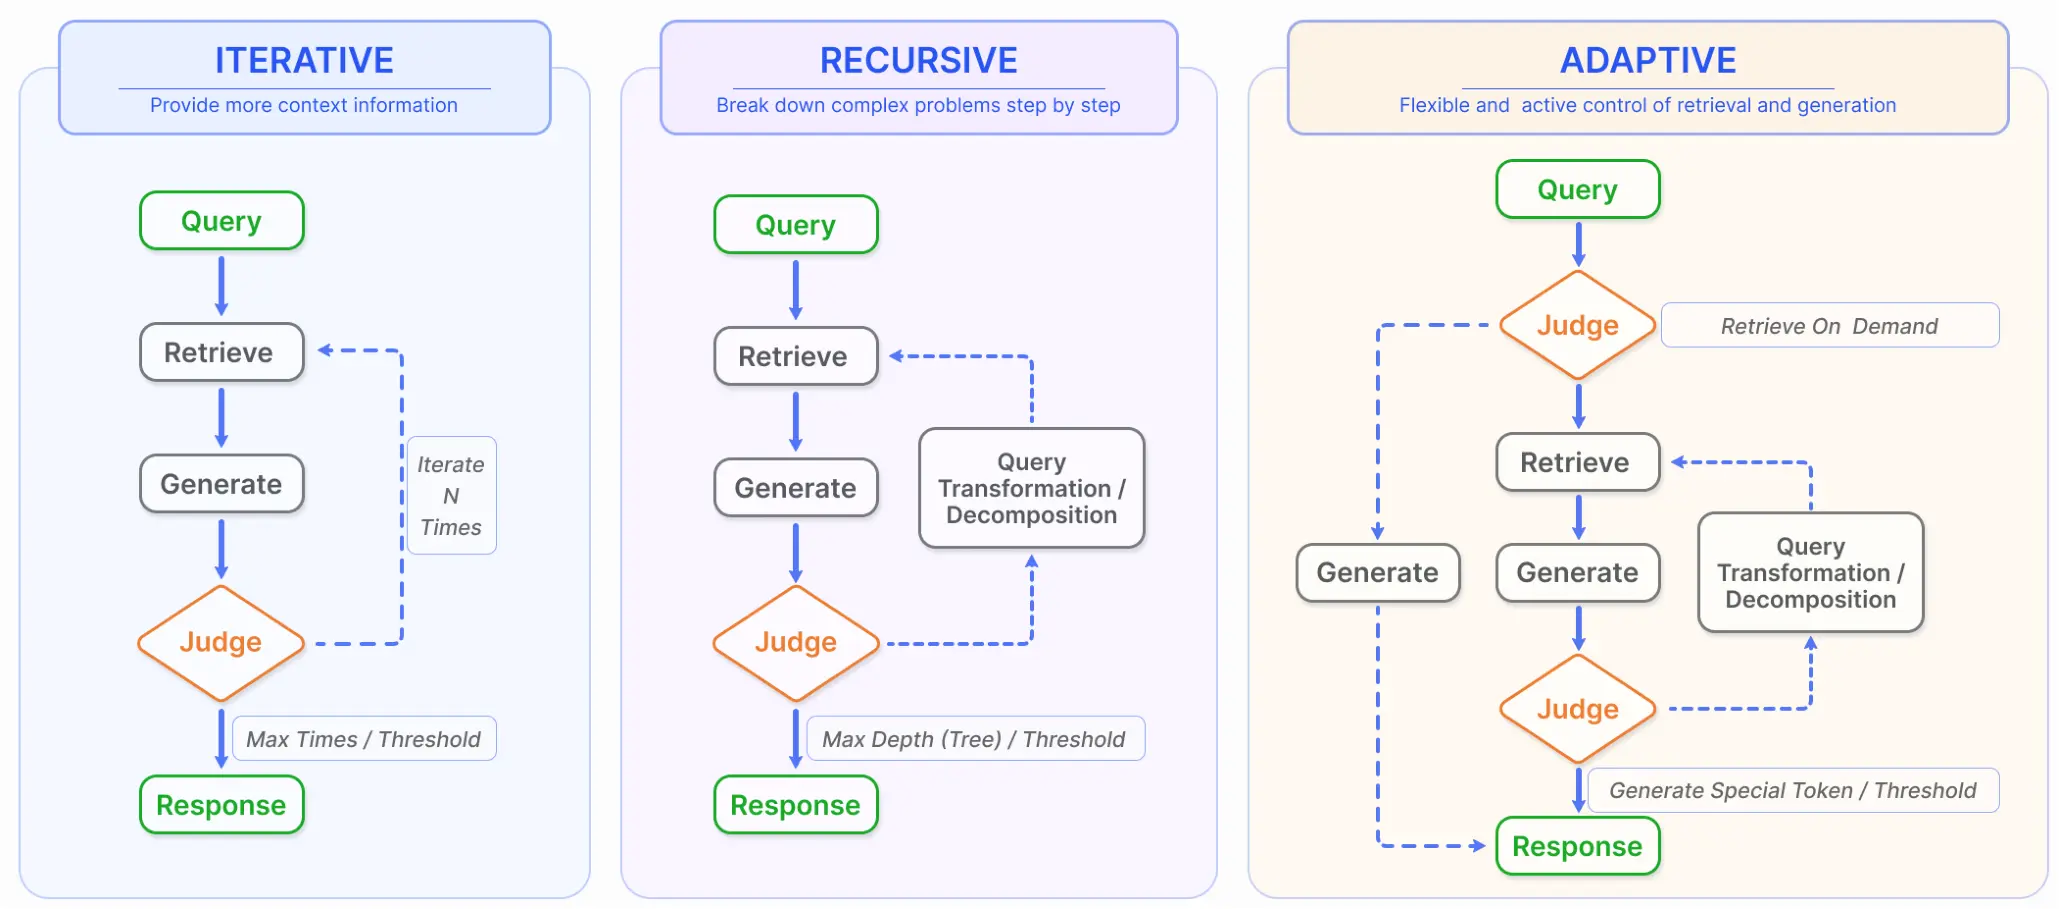
\includegraphics[width=0.9\textwidth]{images/llms/augmentation-process.png}
    \caption{In addition to the most common once retrieval, RAG also includes three types of retrieval augmentation processes. (Left) Iterative retrieval involves alternating between retrieval and generation, allowing for richer and more targeted context from the knowledge base at each step. (Middle) Recursive retrieval involves gradually refining the user query and breaking down the problem into sub-problems, then continuously solving complex problems through retrieval and generation. (Right) Adaptive retrieval focuses on enabling the RAG system to autonomously determine whether external knowledge retrieval is necessary and when to stop retrieval and generation, often utilizing LLM-generated special tokens for control. \textit{Source:} \cite{gao2023retrieval}}
    \label{fig:rag_augmentation}
\end{figure}

In summary, these advanced retrieval strategies—iterative, recursive, and adaptive retrieval—are crucial in addressing the limitations of traditional RAG systems. By refining how and when retrieval occurs, these methods significantly improve the depth, relevance, and accuracy of the information used in generating responses, making RAG systems more capable of handling complex, knowledge-intensive tasks.

\subsection{Future Prospects of RAG Technology}

The field of Retrieval-Augmented Generation (RAG) has seen significant advancements, yet several challenges and opportunities for further research remain. This section discusses the future prospects of RAG technology, focusing on its potential developments and the challenges that must be addressed.

\subsubsection{RAG and Long Contexts}

As research into Large Language Models (LLMs) continues to evolve, the ability of these models to handle increasingly long contexts has improved dramatically. Modern LLMs can effectively handle contexts up to 32,000 tokens, with the industry now moving towards managing contexts of up to 128,000 tokens—equivalent to the length of a 250-page book \cite{ibm2023}. This capability raises questions about the continued relevance of RAG, particularly in tasks such as long-document question answering, where it might seem feasible to input entire documents directly into the model. However, RAG retains its value for several reasons. Firstly, providing an LLM with an excessive amount of context in a single prompt can severely impact inference speed, whereas chunked retrieval and on-demand input significantly enhance operational efficiency. Secondly, RAG-based generation allows for the quick location of original references, enabling users to verify the generated answers. The entire retrieval and reasoning process in RAG is transparent, unlike generation that relies solely on long contexts, which remains a black box. The expansion of context capabilities also opens new avenues for RAG, particularly in tackling complex integrative tasks that require synthesizing information from extensive material. Developing new RAG methods for super-long contexts represents a promising area of future research \cite{gao2023retrieval}.

\subsubsection{Enhancing RAG Robustness}

The presence of noise or contradictory information in the retrieved documents can negatively impact the quality of RAG outputs, leading to the adage that "misinformation can be worse than no information at all." Studies have shown that including irrelevant documents can paradoxically improve accuracy by over 30\%, contradicting the assumption that such inclusion would reduce quality. These findings highlight the need for specialized strategies that integrate retrieval with language generation models more effectively \cite{cuconasu2024power}. Addressing the robustness of RAG systems in the face of noisy or misleading data remains a critical challenge for future research.

\subsubsection{Hybrid Approaches: Combining RAG with Fine-Tuning}

Integrating RAG with fine-tuning techniques is emerging as a powerful strategy for improving model performance. Future research should explore the optimal ways to combine RAG and fine-tuning, whether through sequential, alternating, or end-to-end joint training approaches \cite{lin2023ra}. Another promising avenue is the incorporation of smaller, specialized language models (SLMs) within the RAG framework, where these models can be fine-tuned based on RAG outcomes. For instance, the CRAG model trains a lightweight retrieval evaluator to assess the overall quality of the retrieved documents, triggering different knowledge retrieval actions based on confidence levels \cite{yan2024corrective}. These hybrid approaches offer exciting possibilities for enhancing the efficiency and effectiveness of RAG systems.

\subsubsection{Production-Ready RAG}

The practical application of RAG technology in production environments presents several engineering challenges that must be addressed to enhance its adoption. Key areas of focus include improving retrieval efficiency, enhancing document recall in large knowledge bases, and ensuring data security—such as preventing the inadvertent disclosure of sensitive information by LLMs \cite{alon2022neuro}. The development of the RAG ecosystem is heavily influenced by advancements in its technical stack. Tools like LangChain and LLamaIndex have become integral components of the RAG landscape, offering extensive APIs and user-friendly interfaces. As RAG continues to evolve, there is a clear trend toward specialization, customization, and simplification of RAG tools and platforms.

In chapter 4 of this thesis, I will delve into a case study of RAG application in a production environment by examining WISE, a proprietary chatbot developed by HPA. WISE utilizes the Retrieval-Augmented Generation (RAG) framework to significantly enhance its information retrieval capabilities, offering a sophisticated and efficient solution across various applications. This showcases the effectiveness and reliability of RAG solutions in today’s business landscape.

\subsubsection{Multi-Modal RAG}

RAG technology is rapidly evolving beyond text-based applications to incorporate multi-modal data, resulting in the creation of innovative models that integrate RAG concepts across various domains. In image processing, audio, video, and even code-related tasks, RAG is being used to enhance capabilities such as retrieval, generation, and automatic processing. This expansion into multi-modal domains marks a significant advancement in the development and application of RAG technology, broadening its impact and utility across diverse fields \cite{gao2023retrieval}.

The future prospects of RAG technology are both promising and complex. As RAG continues to evolve, it will be essential to address the challenges of robustness, scaling, and production readiness while exploring new frontiers in multi-modal applications. The ongoing development of hybrid approaches and the potential for breakthroughs in scaling laws offer exciting opportunities for advancing RAG systems. With continued research and innovation, RAG technology is poised to become an even more integral part of the AI landscape, enabling more efficient, accurate, and versatile applications across a wide range of domains.

\section{Future Prospects of LLMs: Beyond the Transformer Architecture}

As the field of AI continues to advance, particularly in the areas of Natural Language Generation (NLG) and Retrieval-Augmented Generation (RAG), the underlying architectures powering these models are increasingly coming under scrutiny. As discussed in the previous sections, the Transformer architecture has been the cornerstone of many state-of-the-art AI models, including LLMs, celebrated for its scalability and ability to handle a wide range of tasks with high efficiency. However, its quadratic inference cost and limitations in handling long-range dependencies have prompted researchers to explore new architectures that might eventually surpass the Transformer.

Despite its dominance, the Transformer architecture is not without its weaknesses. Chief among these is its quadratic scaling with respect to sequence length, which significantly increases computational costs as the input size grows. This limitation becomes particularly pronounced in tasks that require processing long documents or entire books, where maintaining long-range dependencies is crucial for accurate text embeddings and summaries. The challenge, therefore, lies in developing architectures that can achieve sub-quadratic inference times while maintaining the ability to scale to the massive parameter sizes required for state-of-the-art LLMs \cite{paull2023transformer}.

Two emerging architectures, Mamba and BASED, have shown potential in addressing some of these challenges. The Mamba architecture, building on advances in State Space Models (SSM), excels in maintaining and memorizing long-range dependencies—an area where Transformers fall short outside their context window. However, Mamba faces challenges in training efficiency, particularly due to its reliance on operations not optimized for modern GPU hardware, and the complexity of its backpropagation process. These hurdles suggest that while Mamba has significant promise, further research is needed to optimize its performance for large-scale LLM applications \cite{gu2023mamba}.

The BASED architecture, in contrast, combines short-range convolution with long-range Taylor-series attention, offering strong Associative Recall (AR) capabilities—something that has been a weakness for many Transformer challengers. BASED is also designed to run efficiently on existing GPU hardware and can be parallelized for training, making it a more practical contender for large-scale implementation. Its potential for sub-quadratic inference and compatibility with traditional Transformer computation methods positions BASED as a particularly attractive alternative, though it too has yet to be tested at the scale of LLMs like ChatGPT or Gemini \cite{arora2023based}.

While both Mamba and BASED present exciting possibilities, it is unlikely that the Transformer will be dethroned in the immediate future. The current infrastructure, research momentum, and the immense costs associated with training new LLMs around these architectures suggest that the Transformer will remain the dominant architecture for some time. However, the exploration of Mamba and BASED points to a future where AI architectures are more versatile, efficient, and capable of handling increasingly complex tasks.

In conclusion, as the development of LLMs and RAG systems progresses, the potential for new architectures like Mamba and BASED to overcome the limitations of the Transformer offers a glimpse into the future of AI. While these architectures may not yet be ready to replace the Transformer at the core of LLMs, they represent critical steps toward more efficient and powerful AI models. The ongoing research in this area will be essential in shaping the next generation of AI technologies, paving the way for models that can more effectively meet the demands of both current and future applications.

